% Options for packages loaded elsewhere
\PassOptionsToPackage{unicode}{hyperref}
\PassOptionsToPackage{hyphens}{url}
\PassOptionsToPackage{dvipsnames,svgnames,x11names}{xcolor}
%
\documentclass[
]{article}

\usepackage{amsmath,amssymb}
\usepackage{iftex}
\ifPDFTeX
  \usepackage[T1]{fontenc}
  \usepackage[utf8]{inputenc}
  \usepackage{textcomp} % provide euro and other symbols
\else % if luatex or xetex
  \usepackage{unicode-math}
  \defaultfontfeatures{Scale=MatchLowercase}
  \defaultfontfeatures[\rmfamily]{Ligatures=TeX,Scale=1}
\fi
\usepackage{lmodern}
\ifPDFTeX\else  
    % xetex/luatex font selection
\fi
% Use upquote if available, for straight quotes in verbatim environments
\IfFileExists{upquote.sty}{\usepackage{upquote}}{}
\IfFileExists{microtype.sty}{% use microtype if available
  \usepackage[]{microtype}
  \UseMicrotypeSet[protrusion]{basicmath} % disable protrusion for tt fonts
}{}
\makeatletter
\@ifundefined{KOMAClassName}{% if non-KOMA class
  \IfFileExists{parskip.sty}{%
    \usepackage{parskip}
  }{% else
    \setlength{\parindent}{0pt}
    \setlength{\parskip}{6pt plus 2pt minus 1pt}}
}{% if KOMA class
  \KOMAoptions{parskip=half}}
\makeatother
\usepackage{xcolor}
\usepackage[top = 1in,bottom = 1in,left = 1in,right = 1in]{geometry}
\setlength{\emergencystretch}{3em} % prevent overfull lines
\setcounter{secnumdepth}{-\maxdimen} % remove section numbering
% Make \paragraph and \subparagraph free-standing
\makeatletter
\ifx\paragraph\undefined\else
  \let\oldparagraph\paragraph
  \renewcommand{\paragraph}{
    \@ifstar
      \xxxParagraphStar
      \xxxParagraphNoStar
  }
  \newcommand{\xxxParagraphStar}[1]{\oldparagraph*{#1}\mbox{}}
  \newcommand{\xxxParagraphNoStar}[1]{\oldparagraph{#1}\mbox{}}
\fi
\ifx\subparagraph\undefined\else
  \let\oldsubparagraph\subparagraph
  \renewcommand{\subparagraph}{
    \@ifstar
      \xxxSubParagraphStar
      \xxxSubParagraphNoStar
  }
  \newcommand{\xxxSubParagraphStar}[1]{\oldsubparagraph*{#1}\mbox{}}
  \newcommand{\xxxSubParagraphNoStar}[1]{\oldsubparagraph{#1}\mbox{}}
\fi
\makeatother


\providecommand{\tightlist}{%
  \setlength{\itemsep}{0pt}\setlength{\parskip}{0pt}}\usepackage{longtable,booktabs,array}
\usepackage{calc} % for calculating minipage widths
% Correct order of tables after \paragraph or \subparagraph
\usepackage{etoolbox}
\makeatletter
\patchcmd\longtable{\par}{\if@noskipsec\mbox{}\fi\par}{}{}
\makeatother
% Allow footnotes in longtable head/foot
\IfFileExists{footnotehyper.sty}{\usepackage{footnotehyper}}{\usepackage{footnote}}
\makesavenoteenv{longtable}
\usepackage{graphicx}
\makeatletter
\newsavebox\pandoc@box
\newcommand*\pandocbounded[1]{% scales image to fit in text height/width
  \sbox\pandoc@box{#1}%
  \Gscale@div\@tempa{\textheight}{\dimexpr\ht\pandoc@box+\dp\pandoc@box\relax}%
  \Gscale@div\@tempb{\linewidth}{\wd\pandoc@box}%
  \ifdim\@tempb\p@<\@tempa\p@\let\@tempa\@tempb\fi% select the smaller of both
  \ifdim\@tempa\p@<\p@\scalebox{\@tempa}{\usebox\pandoc@box}%
  \else\usebox{\pandoc@box}%
  \fi%
}
% Set default figure placement to htbp
\def\fps@figure{htbp}
\makeatother
% definitions for citeproc citations
\NewDocumentCommand\citeproctext{}{}
\NewDocumentCommand\citeproc{mm}{%
  \begingroup\def\citeproctext{#2}\cite{#1}\endgroup}
\makeatletter
 % allow citations to break across lines
 \let\@cite@ofmt\@firstofone
 % avoid brackets around text for \cite:
 \def\@biblabel#1{}
 \def\@cite#1#2{{#1\if@tempswa , #2\fi}}
\makeatother
\newlength{\cslhangindent}
\setlength{\cslhangindent}{1.5em}
\newlength{\csllabelwidth}
\setlength{\csllabelwidth}{3em}
\newenvironment{CSLReferences}[2] % #1 hanging-indent, #2 entry-spacing
 {\begin{list}{}{%
  \setlength{\itemindent}{0pt}
  \setlength{\leftmargin}{0pt}
  \setlength{\parsep}{0pt}
  % turn on hanging indent if param 1 is 1
  \ifodd #1
   \setlength{\leftmargin}{\cslhangindent}
   \setlength{\itemindent}{-1\cslhangindent}
  \fi
  % set entry spacing
  \setlength{\itemsep}{#2\baselineskip}}}
 {\end{list}}
\usepackage{calc}
\newcommand{\CSLBlock}[1]{\hfill\break\parbox[t]{\linewidth}{\strut\ignorespaces#1\strut}}
\newcommand{\CSLLeftMargin}[1]{\parbox[t]{\csllabelwidth}{\strut#1\strut}}
\newcommand{\CSLRightInline}[1]{\parbox[t]{\linewidth - \csllabelwidth}{\strut#1\strut}}
\newcommand{\CSLIndent}[1]{\hspace{\cslhangindent}#1}

\usepackage{orcidlink}
\usepackage{marvosym}
\makeatletter
\@ifpackageloaded{tcolorbox}{}{\usepackage[skins,breakable]{tcolorbox}}
\@ifpackageloaded{fontawesome5}{}{\usepackage{fontawesome5}}
\definecolor{quarto-callout-color}{HTML}{909090}
\definecolor{quarto-callout-note-color}{HTML}{0758E5}
\definecolor{quarto-callout-important-color}{HTML}{CC1914}
\definecolor{quarto-callout-warning-color}{HTML}{EB9113}
\definecolor{quarto-callout-tip-color}{HTML}{00A047}
\definecolor{quarto-callout-caution-color}{HTML}{FC5300}
\definecolor{quarto-callout-color-frame}{HTML}{acacac}
\definecolor{quarto-callout-note-color-frame}{HTML}{4582ec}
\definecolor{quarto-callout-important-color-frame}{HTML}{d9534f}
\definecolor{quarto-callout-warning-color-frame}{HTML}{f0ad4e}
\definecolor{quarto-callout-tip-color-frame}{HTML}{02b875}
\definecolor{quarto-callout-caution-color-frame}{HTML}{fd7e14}
\makeatother
\makeatletter
\@ifpackageloaded{caption}{}{\usepackage{caption}}
\AtBeginDocument{%
\ifdefined\contentsname
  \renewcommand*\contentsname{Table of contents}
\else
  \newcommand\contentsname{Table of contents}
\fi
\ifdefined\listfigurename
  \renewcommand*\listfigurename{List of Figures}
\else
  \newcommand\listfigurename{List of Figures}
\fi
\ifdefined\listtablename
  \renewcommand*\listtablename{List of Tables}
\else
  \newcommand\listtablename{List of Tables}
\fi
\ifdefined\figurename
  \renewcommand*\figurename{Figure}
\else
  \newcommand\figurename{Figure}
\fi
\ifdefined\tablename
  \renewcommand*\tablename{Table}
\else
  \newcommand\tablename{Table}
\fi
}
\@ifpackageloaded{float}{}{\usepackage{float}}
\floatstyle{ruled}
\@ifundefined{c@chapter}{\newfloat{codelisting}{h}{lop}}{\newfloat{codelisting}{h}{lop}[chapter]}
\floatname{codelisting}{Listing}
\newcommand*\listoflistings{\listof{codelisting}{List of Listings}}
\makeatother
\makeatletter
\makeatother
\makeatletter
\@ifpackageloaded{caption}{}{\usepackage{caption}}
\@ifpackageloaded{subcaption}{}{\usepackage{subcaption}}
\makeatother

\usepackage{bookmark}

\IfFileExists{xurl.sty}{\usepackage{xurl}}{} % add URL line breaks if available
\urlstyle{same} % disable monospaced font for URLs
\hypersetup{
  pdftitle={Balancing Situated and Objective Representations in Archaeological Fieldwork},
  pdfauthor={Zachary Batist},
  pdfkeywords={data work, documentation, collaborative experiences},
  colorlinks=true,
  linkcolor={blue},
  filecolor={Maroon},
  citecolor={Blue},
  urlcolor={Blue},
  pdfcreator={LaTeX via pandoc}}


\title{Balancing Situated and Objective Representations in
Archaeological Fieldwork}

\author{
      {Zachary
Batist \orcidlink{0000-0003-0435-508X} \href{mailto:zachary.batist@mcgill.ca}{\Letter}} \\
          McGill University
     \\
  }

\date{2025-05-22}
\begin{document}
\maketitle
\begin{abstract}
Archaeology comprises both systematic and pragmatic attitudes and
processes concerned with the collection and maintenance of data. This
reflects the need to obtain formally-defined data, while also grappling
with the fuzzy and uncertain nature of archaeological encounters,
especially in fieldwork environments. This produces an epistemic
tension, whereby archaeologists struggle to reconcile their desire to
produce concrete outcomes based on objective facts, and their intuitive
understanding that data are in fact products of situated decisions and
actions. Through observations of archaeological practices, interviews
with archaeologists at work, and analysis of the documents they produced
while recording objects of archaeological concern, this paper
articulates how archaeologists cope with this tension and integrate it
into their work experiences.
\end{abstract}


\begin{tcolorbox}[enhanced jigsaw, breakable, left=2mm, opacityback=0, bottomtitle=1mm, leftrule=.75mm, title=\textcolor{quarto-callout-note-color}{\faInfo}\hspace{0.5em}{Note}, opacitybacktitle=0.6, colbacktitle=quarto-callout-note-color!10!white, arc=.35mm, toptitle=1mm, bottomrule=.15mm, colframe=quarto-callout-note-color-frame, titlerule=0mm, toprule=.15mm, colback=white, coltitle=black, rightrule=.15mm]

This is a preprint of a paper accepted for publication in
\href{https://www.cambridge.org/core/journals/advances-in-archaeological-practice}{Advances
in Archaeological Practice}.

\end{tcolorbox}

\section{Introduction}\label{introduction}

The series of challenges pertaining to the organization, sharing and
reuse of archaeological data, which are often collectively referred to
as the discipline's ``curation crisis'' or ``data deluge'', have
highlighted the wide array of practices that underlie data's
construction, management, dissemination and reuse (Bevan 2012; Huggett
2022a, 2022b). Numerous studies have complicated the common imagination
of data -- which considers them as concise, corpuscular, discrete and
inherently truthful records -- by demonstrating how, in practice, they
are actually messy, incomplete and non-reductive (cf. Batist 2024;
Dallas 2015; Huggett 2022b; Voss 2012). In fact, archaeologists create
data while anticipating their utility as records that inform certain
kinds of analysis, while those who apply data in analytical contexts
simultaneously reconcile their own use-cases with the conditions under
which the data were originally created (Dallas 2015: 190-191).

This is reflected in the ways in which archaeologists reuse data. Faniel
et al. (2013) and Atici et al. (2013) documented how those who reuse
data seek out additional contextual information about the circumstances
of a dataset's creation by communicating directly with the dataset's
originators, thereby establishing a discursive collaborative tie.
Alternatively, many data analysts who operate at a distance from the
contexts in which data originate prefer to trust in the models that give
the data concrete structure, thereby offloading the acts of
reconciliation to those who produced the data (Huggett 2022a). In other
words, reusing data involves establishing trust, which can be garnered
through mutual understanding of the challenges that had to be overcome
to get observations to fit within discrete data structures, or through
reliance on mechanisms of control to ensure that data are collected and
maintained in a consistent manner.

This paper demonstrates some of the strategies employed to establish
trust in data. Through analysis of one illustrative example of
archaeological documentation in fieldwork, I show how data-capture is
not merely a sensory experience whereby nature is recorded on a 1:1
basis, but is in fact structured by models and power relations that
legitimize data and make them useful.

\section{Background}\label{background}

This work builds upon prior studies of archaeological documentation in
fieldwork settings, particularly Edgeworth's (1991: 28) dissertation
that documented ``the transaction between the subject and the object, as
it takes place in the act of discovery,'' which represented an attempt
to ground theoretical discourse concerning the objectivity of the
archaeological record in the practical ``intersubjective work or labour
upon material objects''. This extremely polyvalent work touched on
various aspects of archaeological practice, highlighting the collective
and discursive process of archaeological knowledge production in various
settings. Edgeworth closely examined the physical acts of excavation,
the mindsets of the people doing this work, the sensory and conceptual
apparatus through which objects are uncovered and made meaningful, and
the social transactions that surround and permeate life on the project.
His work drew attention to the social and professional interactions
taking place at an archaeological excavation, and which occur as
archaeologists articulate an object as a meaningful or discrete entity
and make it official. Crucially, Edgeworth highlighted how
archaeological records are produced through improvised, semi-structured
and discursive action, afforded by practical concern and limited by the
prior experiences held by those doing the work.

Similarly, Goodwin (1994, 2010) observed how the formation of concrete
records in fieldwork settings relates to the establishment of
professional frameworks, which lend authoritative legitimacy to the
meanings that archaeologists eventually settled upon. This touched on
similar observations made by Gero (1996), who noted how certain ways of
delimiting features --- which corresponded with gendered experiences ---
were deemed more legitimate than others. Mickel (2021) and Yarrow (2008)
also documented that archaeological labourers (including local labourers
and undergraduate students) are less able to contribute as interpretive
agents in the production of lasting records about the things they
recover.

Thorpe (2012) also argued that the broader social and political
circumstances --- neoliberal austerity, in particular --- in which
archaeological fieldwork tends to operate significantly effects how
interpretations are made and arguments are extended, by effectively
curtailing fieldworkers' creative agency. Huggett (2022a), Caraher
(2019), Batist et al. (2021) and Batist (In review) similarly draw
attention to how digital workflows effectively segregate acts of
recording from acts of analysis and interpretation, by putting
significant epistemic distance between those who hold creative agency in
analytical and interpretive domains and those who occupy the domain of
fieldwork; they further demonstrate how the latter is leveraged by the
former to produce a clear and concise basis upon which formal analytical
methods rest. Moreover, Batist (2024) and Hacıgüzeller, Taylor, and
Perry (2021) point out that the formal and transactional paradigm that
dominates discourse on what data are and how they should be handled
poses problems for communicating what was actually encountered while
excavating a feature, including tentative thoughts, desires and
apprehensions that are left out of official records.

In what follows, I will extend this critique by showcasing the
improvised nature of data construction in fieldwork settings and by
demonstrating how rough encounters with archaeological remains are
stabilized and made more legitimate through documentation practices.

\section{Methods and Materials}\label{methods-and-materials}

This paper draws from observations of and interviews with archaeologists
at work, as well as the documents that they produced. Specifically, I
articulate how archaeologists enacted various activities and how their
actions were situated as part of broader systems of knowledge
production. My involvement with this project constituted a longitudinal
investigation of archaeological practice that contributed to my doctoral
dissertation (see Batist 2023).

\subsection{Case}\label{case}

This paper draws from observations of and interviews with members of an
archaeological project, focusing specifically on the pragmatic and
multifaceted ways in which participants engage with the project's
information system. This involved recording and interviewing
archaeologists as they worked during the summer field seasons from 2017
to 2019 and holding additional interviews between fieldwork sessions.
The project's director also provided access to all documents and records
for the purpose of this research.

The project upon which this case is based is a research project
comprising excavation of a prehistoric site in Southern Europe. It is
directed by a foreign professor affiliated with a North American
university, but who has extensive experience working in the region. The
director coordinates various specialists whom he recruited for their
expertise in the interpretation of finds, a number of trench supervisors
who lead excavation and data collection activities, and excavators who
operate under the guidance of their assigned trench supervisors.

It is a research project involving archaeologists with varying degrees
of experience and coming from diverse professional backgrounds,
including those with extensive experience in the commercial sector (see
the supplementary materials for brief summaries of individuals'
background). It is not a field school, but it does rely to a large
extent on labour provided by undergraduate and graduate students, and as
such engages in on-the-job training. The informal and situated learning
experiences I was able to observe represent instances of legitimate
peripheral participation, whereby newcomers are introduced to the norms
and expectations that govern the archaeological community of practice.
These scenarios provide especially clear opportunities to ascertain the
value ascribed to observed practices and information outcomes conveyed
by teachers and adopted by learners through active and productive
tutelage. There is a strong precedent for this approach to the study of
archaeological practice (cf. Everill 2007; Goodwin 1994, 2010; Morgan
and Wright 2018), including in contexts of continual, life-long learning
among experienced archaeologists (cf. Edgeworth 1991; Gero 1994; Graham
2019).

This project served as one of three cases I investigated for my doctoral
dissertation, which documents how archaeological information systems
scaffold the collaborative and epistemic commitments that govern
professional research practices (Batist 2023). The observations and
elicitations I present in this paper illustrate a specific phenomenon
with a more refined scope than what is accounted for in that more
comprehensive work and in other research outcomes deriving from it (cf.
Batist, In review, 2024; Batist et al. 2021). As such, this paper draws
from a relatively small portion of the entire set of observations and
interviews, which largely pertain to fieldwork recording practices,
processing and analysis of finds, records management, interdisciplinary
collaboration, decisions regarding writing and publication of findings,
and discussions of how data and findings are presented, evaluated and
revised among broader research communities.

I actively contributed to the project for several years, primarily
serving as a database manager. This afforded me with greater awareness
of its organizational and institutional history, including a deeper
familiarity with all the people involved, and provided me with a
privileged outlook on how team members structure information, how they
typically use data, and what circumstantial events or motivating factors
frame such concerns. My continual and participatory engagement with this
project allowed me to develop an understanding of the intricate social
relations as they developed over time, and enabled me to examine certain
methods that are drawn out over the course of several field seasons.

I must emphasize that in case-study research, cases represent discrete
instances of a phenomenon relating to a researcher's interest (Ragin
1992). Cases are therefore not the subjects of inquiry, but the vehicles
through which phenomena of interest are manifested in an observable way.
I recognize that all archaeological projects are informed by their own
histories, memberships, sets of tools, methods, and social or political
circumstances, which inform distinct traditions of practice, and that it
is not possible to generalize across the whole discipline through a
single case study. In other words, my findings are informed by the
informants whose actions and attitudes I sought to articulate, and by my
own perspective as a scholar of the culture and practice of archaeology
and of the media and infrastructures that support it. The implication is
that commercial archaeology, which comprises the vast majority of
archaeological work in North America and Europe, is out of the study's
scope, owing to the fact that the case represents a research project and
that I have very limited experience with and knowledge about commercial
archaeology. However, see Chadwick (1998), Thorpe (2012) and Zorzin
(2015) for similar research pertaining to commercial archaeology which
produced complementary findings as those presented here.

That being said, this single case study does articulate some significant
factors that contribute to decisions and behaviours that archaeologists
commonly make and enact, makes certain underappreciated social and
collaborative commitments that underlie common tools and practices more
visible, and draws attention to certain patterns of practice that relate
to contemporary discourse on the nature of archaeological data and
ongoing development of information infrastructures.

\subsection{Data}\label{data}

My dataset comprises recorded observations, embedded interviews,
retrospective interviews, archaeological documentation, and ethnographic
and reflexive fieldnotes.

Observational data comprised records of participants' behaviours as they
performed various archaeological activities and take the form of video,
audio and textual files. They enable me to document \emph{how} practices
are performed, in addition to the fact \emph{that} they are performed.
Moreover, observational data allow me to document what participants
actually do as opposed to what they think or say they do. For instance,
I situated activities in relation to broader systems, even when
participants are unaware that they are contributing to these systems, in
order to consider how activities occurring at various times or in
various contexts indirectly relate to, compare with or inform each
other. I observed roughly 66 hours of work from this case, which were
typically recorded using three different cameras --- including cameras
placed on participants' foreheads --- to obtain different perspectives
on the recorded activities. Some of the primary foci that guided my
observations were the processes that result in archaeological records;
people's use of information objects or interfaces, which sometimes
differ from expected behaviour established through their design; how
subjects implemented unconventional solutions or ``hacks'' to work
around problems; how the context of an activity affects its
implementation; and how local or idiosyncratic terms, concepts and
gestures become established in a research community.

Embedded interviews comprised conversational inquiries with participants
in the context of their work, and were meant to account for
participants' perspectives regarding how and why they act as they do,
given the immediate constraints of the situation at hand. Embedded
interviews provided insight into the practicalities of work in the
moment, from the perspective of practitioners themselves (Flick 1997,
2000; Witzel 2000). They are also useful for comparing participants'
responses with observational records to interrogate how and why
participants' observed actions may differ from the rationales elucidated
from embedded interviews. The fact that embedded interviews occurred
while observing work practices makes it difficult to distinguish these
interactions from their broader contexts, and it is therefore
impractical to quantify how much data were collected in this way.
Embedded interviews focused on how participants identify problems or
challenges in their work, and to determine ways to resolve them; how
certain people gain recognition as domain experts or authorities with
specialized knowledge; how specialists relate their contributions to the
contributions of others; and how specialists relate their situated
perspectives to centralized knowledge repositories.

Retrospective interviews comprised longer sem-structured interviews
outside of work settings with select participants to contextualize data
collected by other means and to determine participants' views on more
general or relatively unobservable aspects of archaeological research
(such as planning, publishing, collaboration, etc). Participants were
selected for interviews based on the potential to triangulate different
perspectives on objects, themes or situations whose significance was
emerging throughout the research (Morse and Clark 2019). I conducted 13
interviews during this case; some included more than one participant,
and some participants sat for more than one interview. Retrospective
interviews helped me gain insight into how participants situate
themselves as members of and in relation to research communities, which
may be characterized by different regimes of value and by different
methodological protocols or argumentation strategies. They were meant to
highlight participants' perspectives on the value of various kinds of
research outputs, what they value in their work and the work of others,
the major constraints and challenges that they and their communities
face, and how they might resolve them.

I examined documents and media (such as forms, photographs, labels,
databases, datasets, reports, instructional media and field manuals) to
gain insight into institutional norms or expectations. See Batist (2024)
and Batist (In review) for more in-depth analysis of how people
interacted with and valued these documents. This involved examining
documents and media as means for encapsulating and communicating
meanings among users across space and over time. This helped me to
understand the vectors through which participants either tacitly form
collective experiences or directly collaborate among themselves (Huvila
2011, 2016; Yarrow 2008). Document analysis emphasized understanding how
document design and media capture protocols anticipate certain methods;
how various activities refer to recorded information; the reasons why
team members ignore certain equipment and forms of documentation despite
their availability; how record-keeping is controlled through explicit or
implicit imposition of limitations or constraints; why certain records
play a more central role than others; and how different archaeologists
record the same objects in different ways.

Finally, my field notes comprised reflexive journal entries that I wrote
between observational sessions or interviews. They also include moments
from observational sessions or interviews that I deemed particularly
important, as well as descriptive accounts of unrecorded activities or
conversations that I have since deemed useful data in their own right.

I obtained informed consent from all individuals included in this study
in compliance with the University of Toronto's Social Sciences,
Humanities, and Education Research Ethics Board, Protocol 34526. In
order to ensure that participants could speak freely about their
personal and professional relationships while minimizing risk to their
personal and professional reputations, I committed to refrain from
publishing any personally identifying information. I refer to all
participants, affiliated organizations, and mentioned individuals or
organizations using pseudonyms. I also edited visual media to obscure
participants' faces and other information that might reveal their
identities, and took care to edit or avoid using direct quotations that
were cited in other published work that follows a more permissive
protocol regarding the dissemination of participants' identifying
information.

\subsection{Analysis}\label{analysis}

I analyzed recorded observations and interviews, and interrogated the
roles and affordances of various tools and documents, using qualitative
data analysis methods. More specifically, I draw from the
``constellation of methods'' that Charmaz (2014: 14-15) associated with
grounded theory, namely coding and memoing. Coding involves defining
what data are about in terms (or codes) that are relevant to the
theoretical frameworks that inform my research, and identifying
instances of these concepts (codings) as they appear throughout the text
(Charmaz 2014: 43). Memoing entails more open-ended exploration and
reflection upon latent ideas in order to crystallize them into new
avenues to pursue, and constitutes a relatively flexible way of engaging
with data and serves as fertile ground for honing new ideas (Charmaz
2014: 72). By creating memos that relate and elaborate series of encoded
observations and that situate observed experiences in relation to
broader theoretical frameworks, I was able to form more robust and
thematic arguments about the phenomena of interest while remaining
firmly grounded in the empirical data. See Batist (2024: 9-10) for a
more comprehensive overview of the analytical methods employed for the
project from which this paper emerges.

Codes were generated through iterative analysis of recorded
observations, transcribed interviews and scans of documents and field
notes. An initial ``open'' coding phase involved generating codes in a
rather open-ended manner to identify common themes and sensitizing
concepts (Bowen 2006; Charmaz 2014: 30-31). Subsequent coding was
scaffolded by a provisional taxonomic code system, which was informed by
a loose conceptual model, which broadly encompasses codes about specific
activities, participants' figurations, and theoretical concepts
concerning the collective constitution of scientific knowledge (see
Batist 2023: Appendix B for an overview of the code system). The study
is therefore aligned with Charmaz's (2000) constructivist approach to
grounded theory, in that it orients the work by the analyst's prior
understandings, rather than have the codes emerge organically.

I refer to specific observations or interview segments throughout the
rest of this text using endnotes, which are indexed in the supplementary
materials.

\section{Findings}\label{findings}

I focus on a string of episodes where Jane, a promising trench assistant
working at an archaeological project, learned to identify,
differentiate, and document parts of a stratigraphic sequence. I
illustrate how the constitution of the archaeological record, and the
internalization of archaeological knowledge, occurred as part of project
frameworks and collaborative relations that were structured by projects'
divisions of labour.

\subsection{Learning to see like an
archaeologist}\label{learning-to-see-like-an-archaeologist}

As illustrated in Figure~\ref{fig-context-change}, Jane explained to me
how she identified and differentiated a new context that she was
beginning to expose in her trench, using a series of gestures paired
with speech to help convey what she meant to
say.\textsuperscript{\hyperref[sec-A1]{A1}} Jane kicked the boulders as
she referred to them, literally pointed out relations to previous
experiences that she deemed relevant, and described certain aspects of
the soil by miming the ways that she would interact with them. She
referred to common nomenclature outlined in the project's standard
recording schema and referenced by more experienced personnel, and drew
from her experiences working in other trenches that others may have
shared. More generally, she described the context change only in terms
of her interactions with it, and as framed by her particular role in the
project.

\begin{figure}

\centering{

\pandocbounded{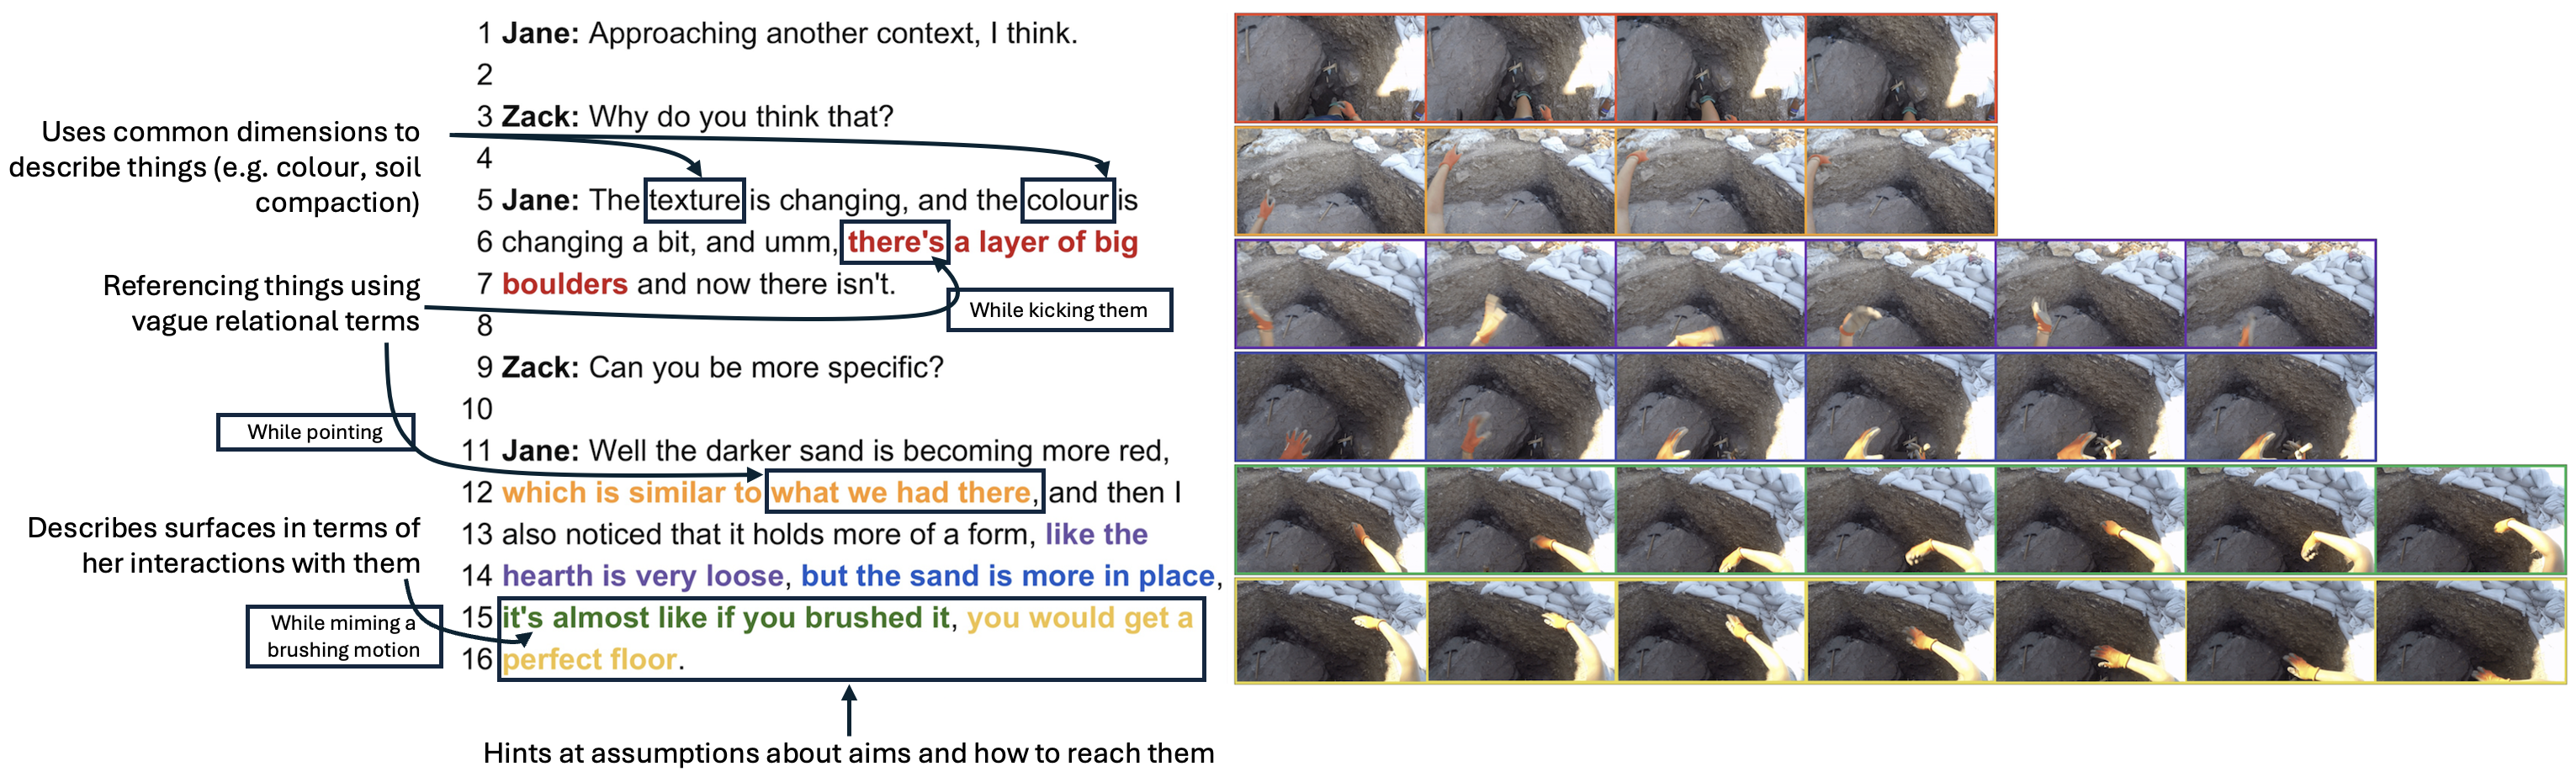
\includegraphics[keepaspectratio]{figures/context-change-annotated.png}}

}

\caption{\label{fig-context-change}Discussion of a potential context
change using gestures and speech.}

\end{figure}%

Afterward, and as illustrated in
Figure~\ref{fig-context-change-discussion}, Jane consulted with Basil,
who supervised work in this trench, and who is also the project
director, regarding her interpretation of the soil in
it.\textsuperscript{\hyperref[sec-A2]{A2}} Jane explained what she saw,
in terms of her encounters with the entities she identified, while
punctuating her observations with physical gestures that underscored
certainty that the entities she was observing actually exist. Basil came
to take a closer look and translated Jane's situated experiences into
more nominal and normalized terms, that distance the observer from the
observed entities. Basil then identified a series of actions that Jane
must implement, and summarized the situation by joining what was
observed with what was to be done about it, in effect rendering a
conclusive and well-reasoned decision. All the while, Jane confirmed her
understanding of Basil's corrections and of his specific instructions.

\begin{figure}

\centering{

\pandocbounded{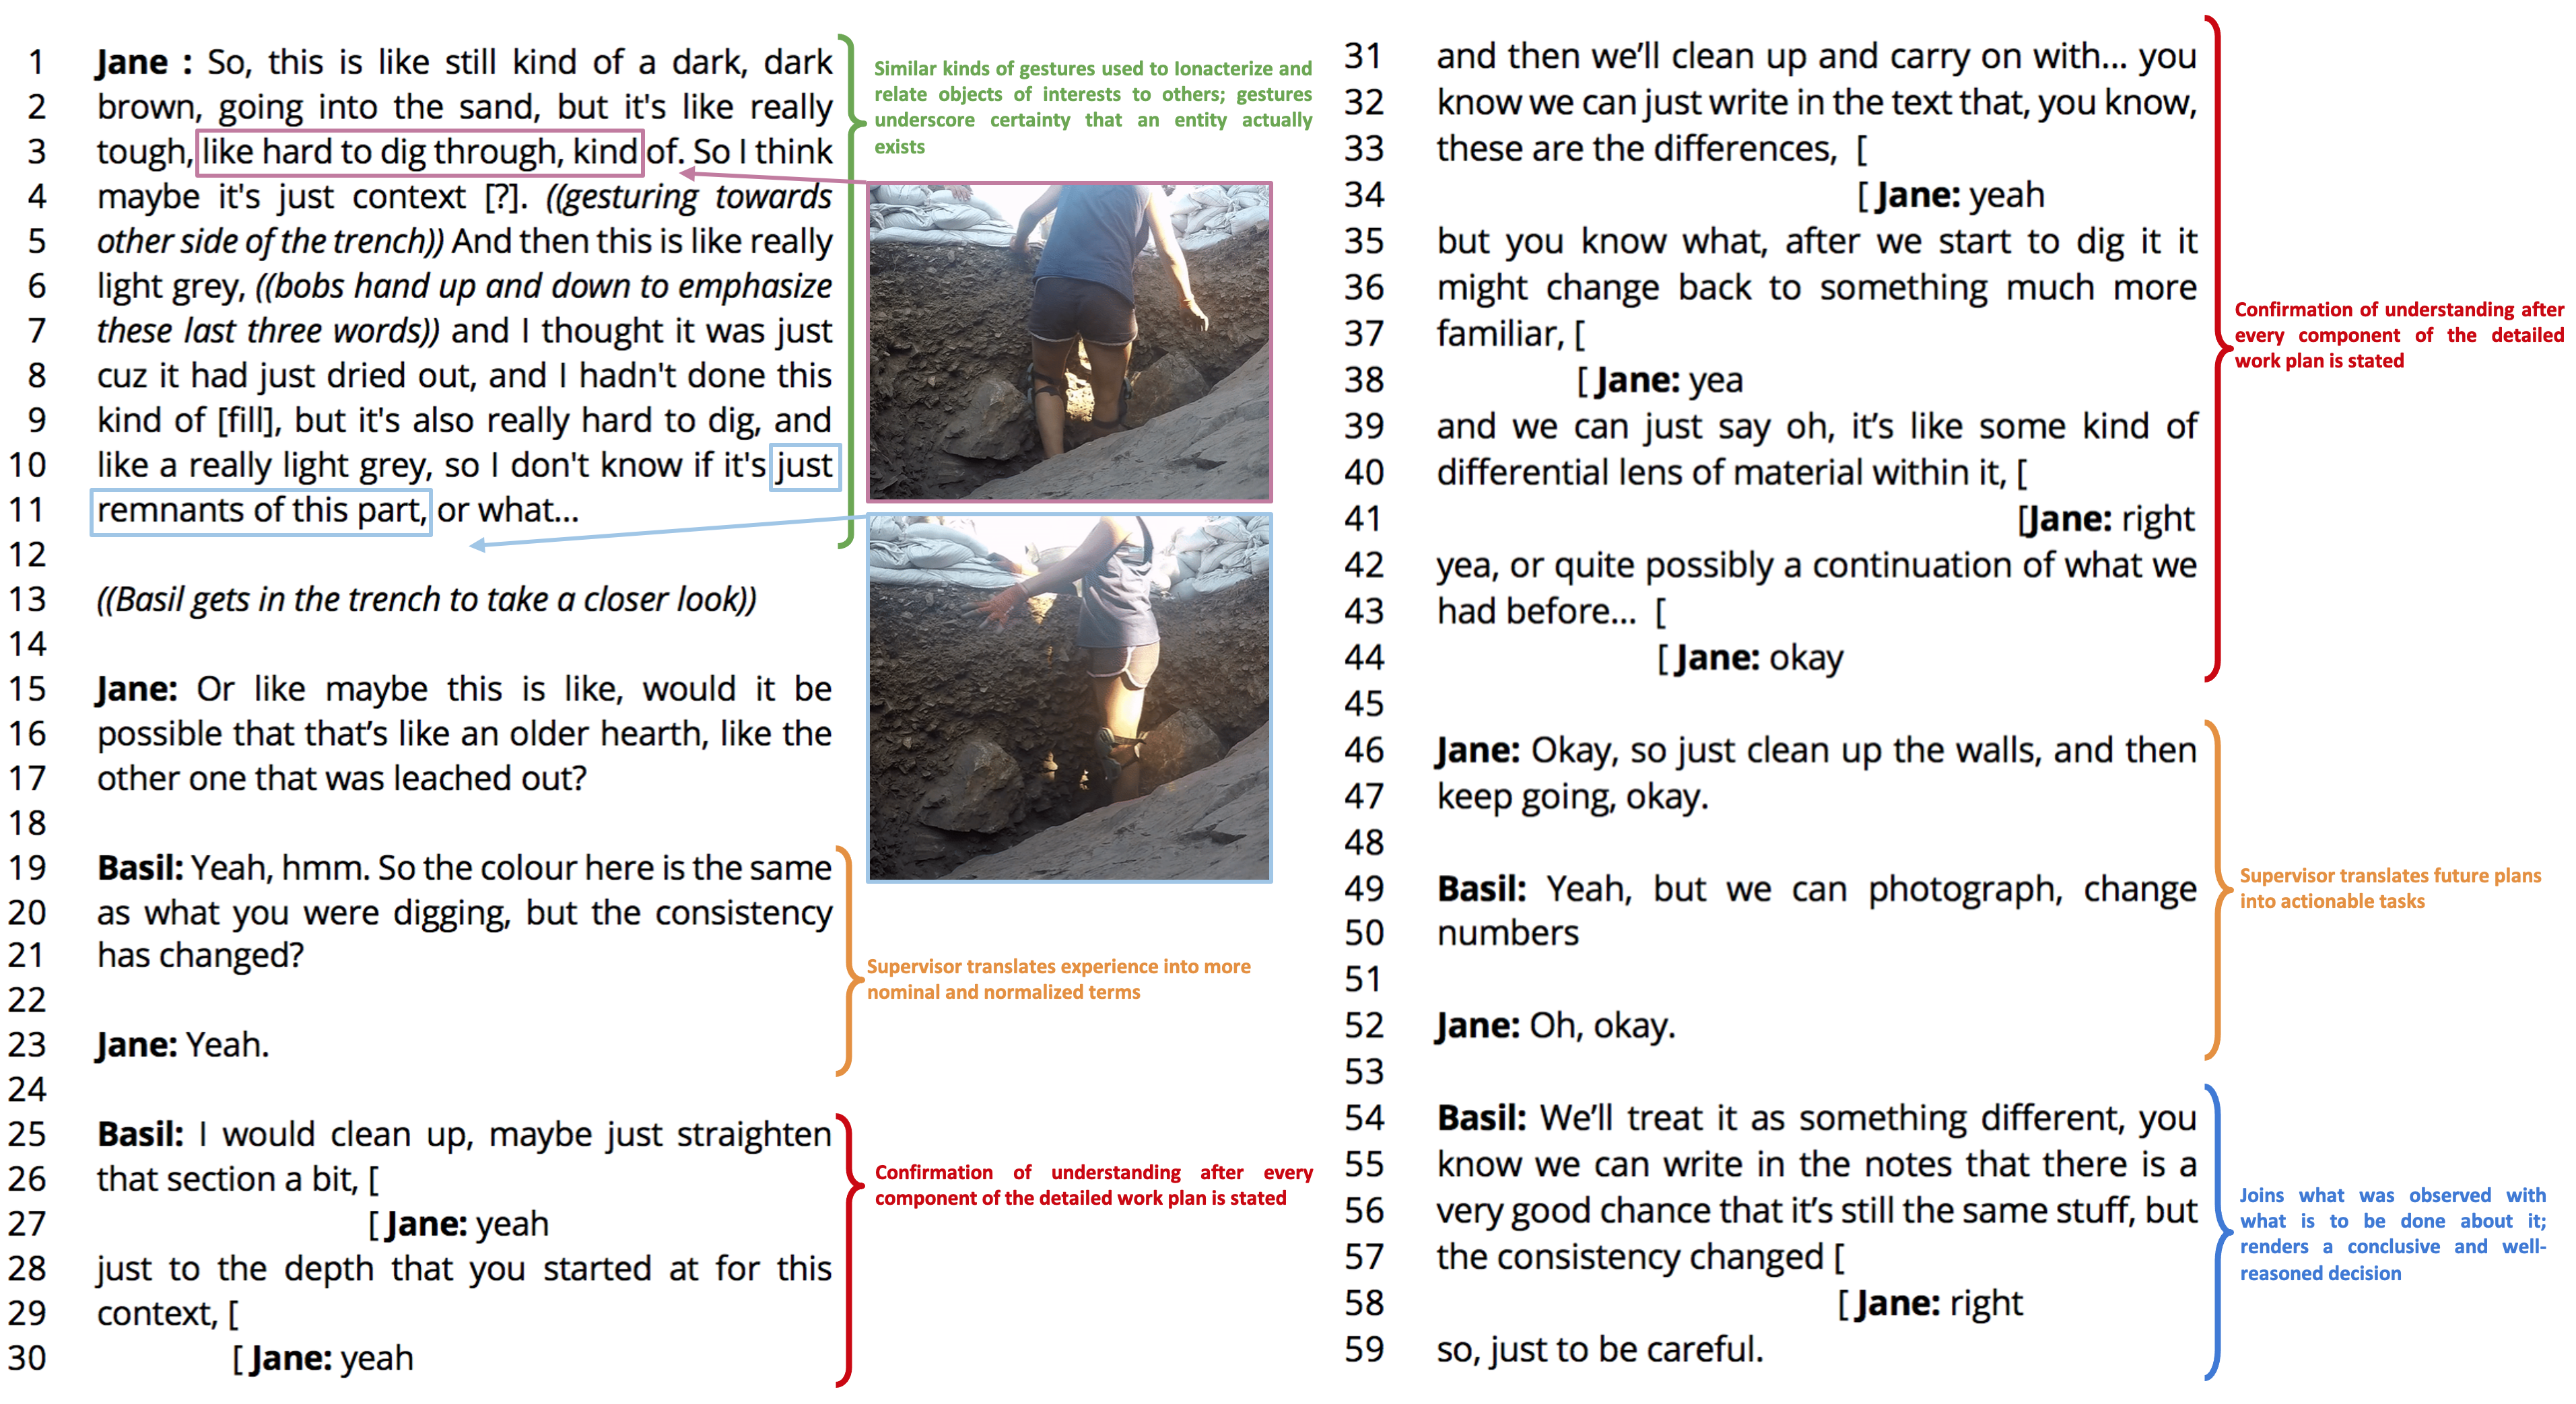
\includegraphics[keepaspectratio]{figures/context-change-discussion.png}}

}

\caption{\label{fig-context-change-discussion}Explanation of a potential
context change using gestures and speech.}

\end{figure}%

When Jane explained her interpretation of the soil to her supervisor, he
then responded with tentative agreement, paired with his own gestures
and intonations that subtly communicated his agreement or disagreement.
The conversation between Jane and Basil therefore served as a means of
calibrating their experiences, using an independent framework as a
common reference point. In effect, Basil attempted to align Jane's
emerging perspective with a professional outlook on the sediment's
character.

As Jane stated in a subsequent interview Figure~\ref{fig-training-eye},
she initially found it difficult to ``train her eye to see what they're
seeing'', and ``they'' seems to refer to more senior and specialized
archaeologists, including her supervisor the director, and Alfred, one
of the field directors.\textsuperscript{\hyperref[sec-A3]{A3}} By
talking through their observations in an explicit manner and in the
presence of the entities of mutual concern, while also referencing
concrete characteristics of the soil, Basil trained Jane to see things
in a way that corresponds to a formal model of how to differentiate
contexts as a natural extension of that ability. This made him more
confident in Jane's ability to recognize and report her experiences,
upon which Basil depends; as he recalled in a separate interview, Basil
came to trust Jane ``to either make her own decisions or be responsible
enough to ask other people to help her make decisions for those moments
when I'm not there.''\textsuperscript{\hyperref[sec-A4]{A4}} This was
because Jane became capable of deciding for herself when and how to
distinguish between sediments, having internalized a conceptual
framework that affords professional legitimacy to her observational
techniques.

\begin{figure}

\centering{

\pandocbounded{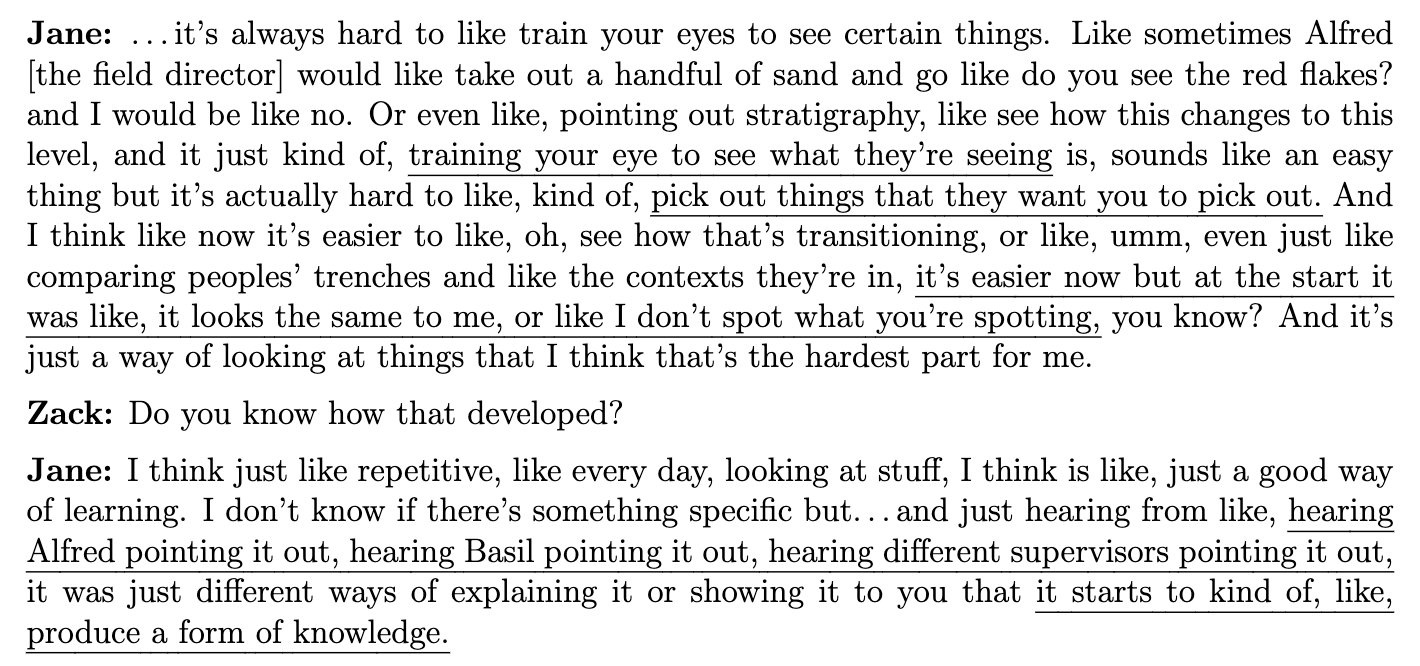
\includegraphics[keepaspectratio]{figures/training-eye.png}}

}

\caption{\label{fig-training-eye}Jane describes how she learned to
recognize differences in the soil. Underlined text refer to especially
significant elicitations elucidated above.}

\end{figure}%

Jane's internalization of the broader conceptual framework accomplished
a few important things: (a) it aligned her own vision as part of a
collectively-held way of perceiving the world, which is led by
authoritative actors who exhibit greater creative control; (b) it
rendered her own unique experiences as generic contributions to the
project's information commons, which has the effect of reducing her
individual agency while also drawing her into a class of related agents
serving similar data collection functions, e.g.~student labourers; and
(c) it re-framed her embodied and sensory experience as a matter of
information modelling, which occurs outside material space and
circumstantial moments in time. By clarifying relatively ambiguous
perceptions through a carefully calibrated prism, the project may obtain
sharper and more well-defined outlines of the things they target for
observation, while correcting for and making it easier to dismiss the
particular embodied experiences that are collectively focused through
the aggregative lens.

\subsection{Shedding the body}\label{shedding-the-body}

I should note that Jane did not actually object to the reduction of her
situated experience in favour of more generic forms of representing the
stratigraphy. In fact, this conformed with a pattern of behaviour ---
which was enacted by all the fieldworkers I spoke with --- whereby they
tried not to think too much while excavating, opting instead to operate
in the moment, face the task at hand, and deal with what is immediately
in front of them, literally and
figuratively.\textsuperscript{\hyperref[sec-A5]{A5},\hyperref[sec-A6]{A6}}
This conformed with the expectation that the things an excavator
uncovers will gradually reveal themselves, and that she should passively
follow what is occurring in the earth before her.

To help accomplish this, fieldworkers modified the environments in which
they worked. For instance, some fieldworkers focused better while
listening to music or while blocking out social
distractions.\textsuperscript{\hyperref[sec-A7]{A7},\hyperref[sec-A8]{A8}}
Ben, who worked as an assistant in a separate trench, said that
listening to music helped him avoid being too
self-aware\textsuperscript{\hyperref[sec-A7]{A7}} while Jane concurred
by expressing that she listened to music to help her ``get lost in
digging.''\textsuperscript{\hyperref[sec-A8]{A8}} Even when music was
not used, or when it is forbidden on site, there remains a warrant for
fieldworkers to remain focused as they
work.\textsuperscript{\hyperref[sec-A9]{A9}} For instance, Basil
recalled what he characterized as ``old fashioned'' archaeological
fieldwork practices, which dictate that ``the only sound you should hear
is trowel on stone.''\textsuperscript{\hyperref[sec-A8]{A8}}

Having all the necessary tools at hand was another way to facilitate
uninterrupted focus during
fieldwork.\textsuperscript{\hyperref[sec-A10]{A10}} This helped
eliminate peripheral sensory distractions when getting up or reaching
for tools placed further away. In effect, fieldworkers were made to
become disembodied sensing devices attuned to one thing and one thing
only: the soil immediately in front of them. This notion was further
underscored by my unrecorded but common observations of supervisors
having to force assistants to take breaks, drink water, apply sunscreen,
and remind them that they have bodies worth cherishing and protecting.

In some cases, fieldworkers found certain kinds of externally derived
information useful as they excavated. For instance, knowing about
similar stratigraphy in nearby trenches enabled excavators to work at a
quicker pace, since it this provided a general understanding of the
order and depth of the stratigraphy under
them.\textsuperscript{\hyperref[sec-A11]{A11},\hyperref[sec-A12]{A12}}
Moreover, when finds specialists reported back to fieldworkers about the
contents of their ongoing trenches, their preliminary findings sometimes
influenced the care with which they excavated and recorded the
trench.\textsuperscript{\hyperref[sec-A13]{A13},\hyperref[sec-A14]{A14}}
While Theo (a trench supervisor who eventually became a field director)
indicated that knowing about the properties of lithic artifacts that
lithics specialists deemed important helped him undertake his work in a
manner that better suited the project's overall aims, he presented this
notion in very broad terms, and refrained from indicating specific
practical impacts when prompted.
\textsuperscript{\hyperref[sec-A13]{A13}} Moreover, Ben dismissed the
input provided by palaeobotanical experts as useless to him because he
was unable to ``see'' the archaeobotanical traces as he
worked.\textsuperscript{\hyperref[sec-A15]{A15}} This may merely reflect
practical concerns, specifically regarding the microscopic nature of
properties that render archaeobotanical remains significant, but it
would not be absurd to find ways to help fieldworkers make sense of such
insights in the field. For instance, if there was a warrant for such
activity, fieldworkers may hypothetically carry a magnifying loupe and
reference guide, and be trained to understand how to use them, similar
to how Jane learned to characterize soil samples in the field. However,
this would require a more comprehensive partnership between specialists
and fieldworkers, and broadening the extreme focus that fieldworkers
have honed for themselves.

In general then, I observed aspects of fieldwork practice that both
complement and contradict efforts to enhance reflexivity in fieldwork.
The professed desire not to overthink while excavating pushes back
against impulses to provide more information to fieldworkers during the
moment of excavation (cf. Berggren 2012; Berggren et al. 2015).
According to Theo and Ben, fieldworkers operate in a strictly separate
role than those who interpret and write about finds, and this boundary
feels natural to
them.\textsuperscript{\hyperref[sec-A16]{A16},\hyperref[sec-A17]{A17},\hyperref[sec-A18]{A18}}
Rather than ingest loads of additional information, which involves
learning how to make sense of it all and find it meaningful in a
practical sense,\textsuperscript{\hyperref[sec-A19]{A19}} the
fieldworkers I spoke with went in the opposite direction; they value
their extremely focused experiences with the material, which presents
them with a unique and proprietary way of knowing that dissipates as
they are, as Edgeworth (2003: 109) put it, forced to ``{[}detach
themselves{]} from the task-in-hand to consider the material field from
a distance''. This means of engagement feels more natural to them, as if
unmuddied by reflexive thought, and the fieldworkers I spoke with
perceived this as a strength.

At the same time, the fieldworkers I spoke with were very aware that all
observation is subjective and that all records carry biases imposed by
the practical circumstances of their creation; they were deeply involved
in navigating these practical circumstances and in devising ways to
control their environments to foster the \emph{illusion} of objectivity.
All of what I described was in service of a broader systemic framework,
which is informed by a (flawed) conception of the nature of
archaeological data and of what constitutes proper or legitimate
archaeological reasoning (Batist, In review).

In other words, fieldworkers' efforts to shed their embodied experiences
was a strategy for coping with an ``epistemic anxiety'', whereby
archaeologists must grapple with a tension between the drive to produce
confident records and their intuitive understanding that their own
observations are inherently situated (Huggett 2022b: 274-278; Lucas
2019: 55-57; Wylie 2017; Batist 2024). This is supported by systems that
effectively re-assign creative agency from fieldworkers to data managers
(Batist 2024, In review). For instance, I previously noted that database
managers, who were tasked with translating messy observations into
concrete data structures, generally lacked adequate understanding of the
contexts in which data were initially recorded; to overcome this
challenge, they attempted to enforce standards, workflows and rulesets
among fieldworkers so that they could obtain greater control over the
data (Batist 2024).

It should also be emphasized that this is a systemic issue, and does not
reflect individual archaeologists' skills and abilities. This is evident
by the remarkable consistency across responses by and observations of
all the archaeologists I engaged with on this matter, regardless of
their degree of experience; they were all both intuitively and
explicitly aware of these concerns but were unable to grapple with them
or enact change through their own individual actions. Nor are these
observations intended to demonize or pass negative judgement on the
projects' leaders and database managers, who are similarly constrained
by systemic pressures to generate forms of knowledge that are valued by
the scientific enterprise. This, in turn, involves balancing a tension
between sharing concrete records about archaeological observations while
accounting for the situated decisions and actions that contributed their
creation.

\subsection{Leaving traces in the subsequent
record}\label{leaving-traces-in-the-subsequent-record}

Turning back to the specific observations of archaeological fieldwork,
Basil's prediction that the context would not change came to fruition.
However, the tentative decision to proceed as if a change in context was
imminent left residual traces on recording sheets, in the database, and
in the final trench report (see
Figure~\ref{fig-context-description-transcribed} and
Figure~\ref{fig-context-sketch}).

\begin{figure}

\centering{

\pandocbounded{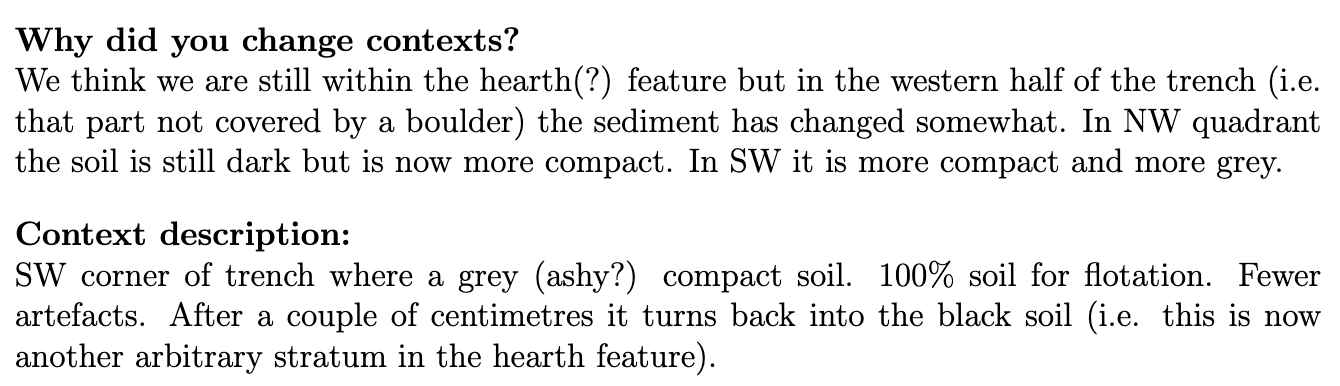
\includegraphics[keepaspectratio]{figures/context-description-transcribed.png}}

}

\caption{\label{fig-context-description-transcribed}Transcribed section
of a recording sheet describing the context addressed in the observed
episode.}

\end{figure}%

\begin{figure}

\centering{

\pandocbounded{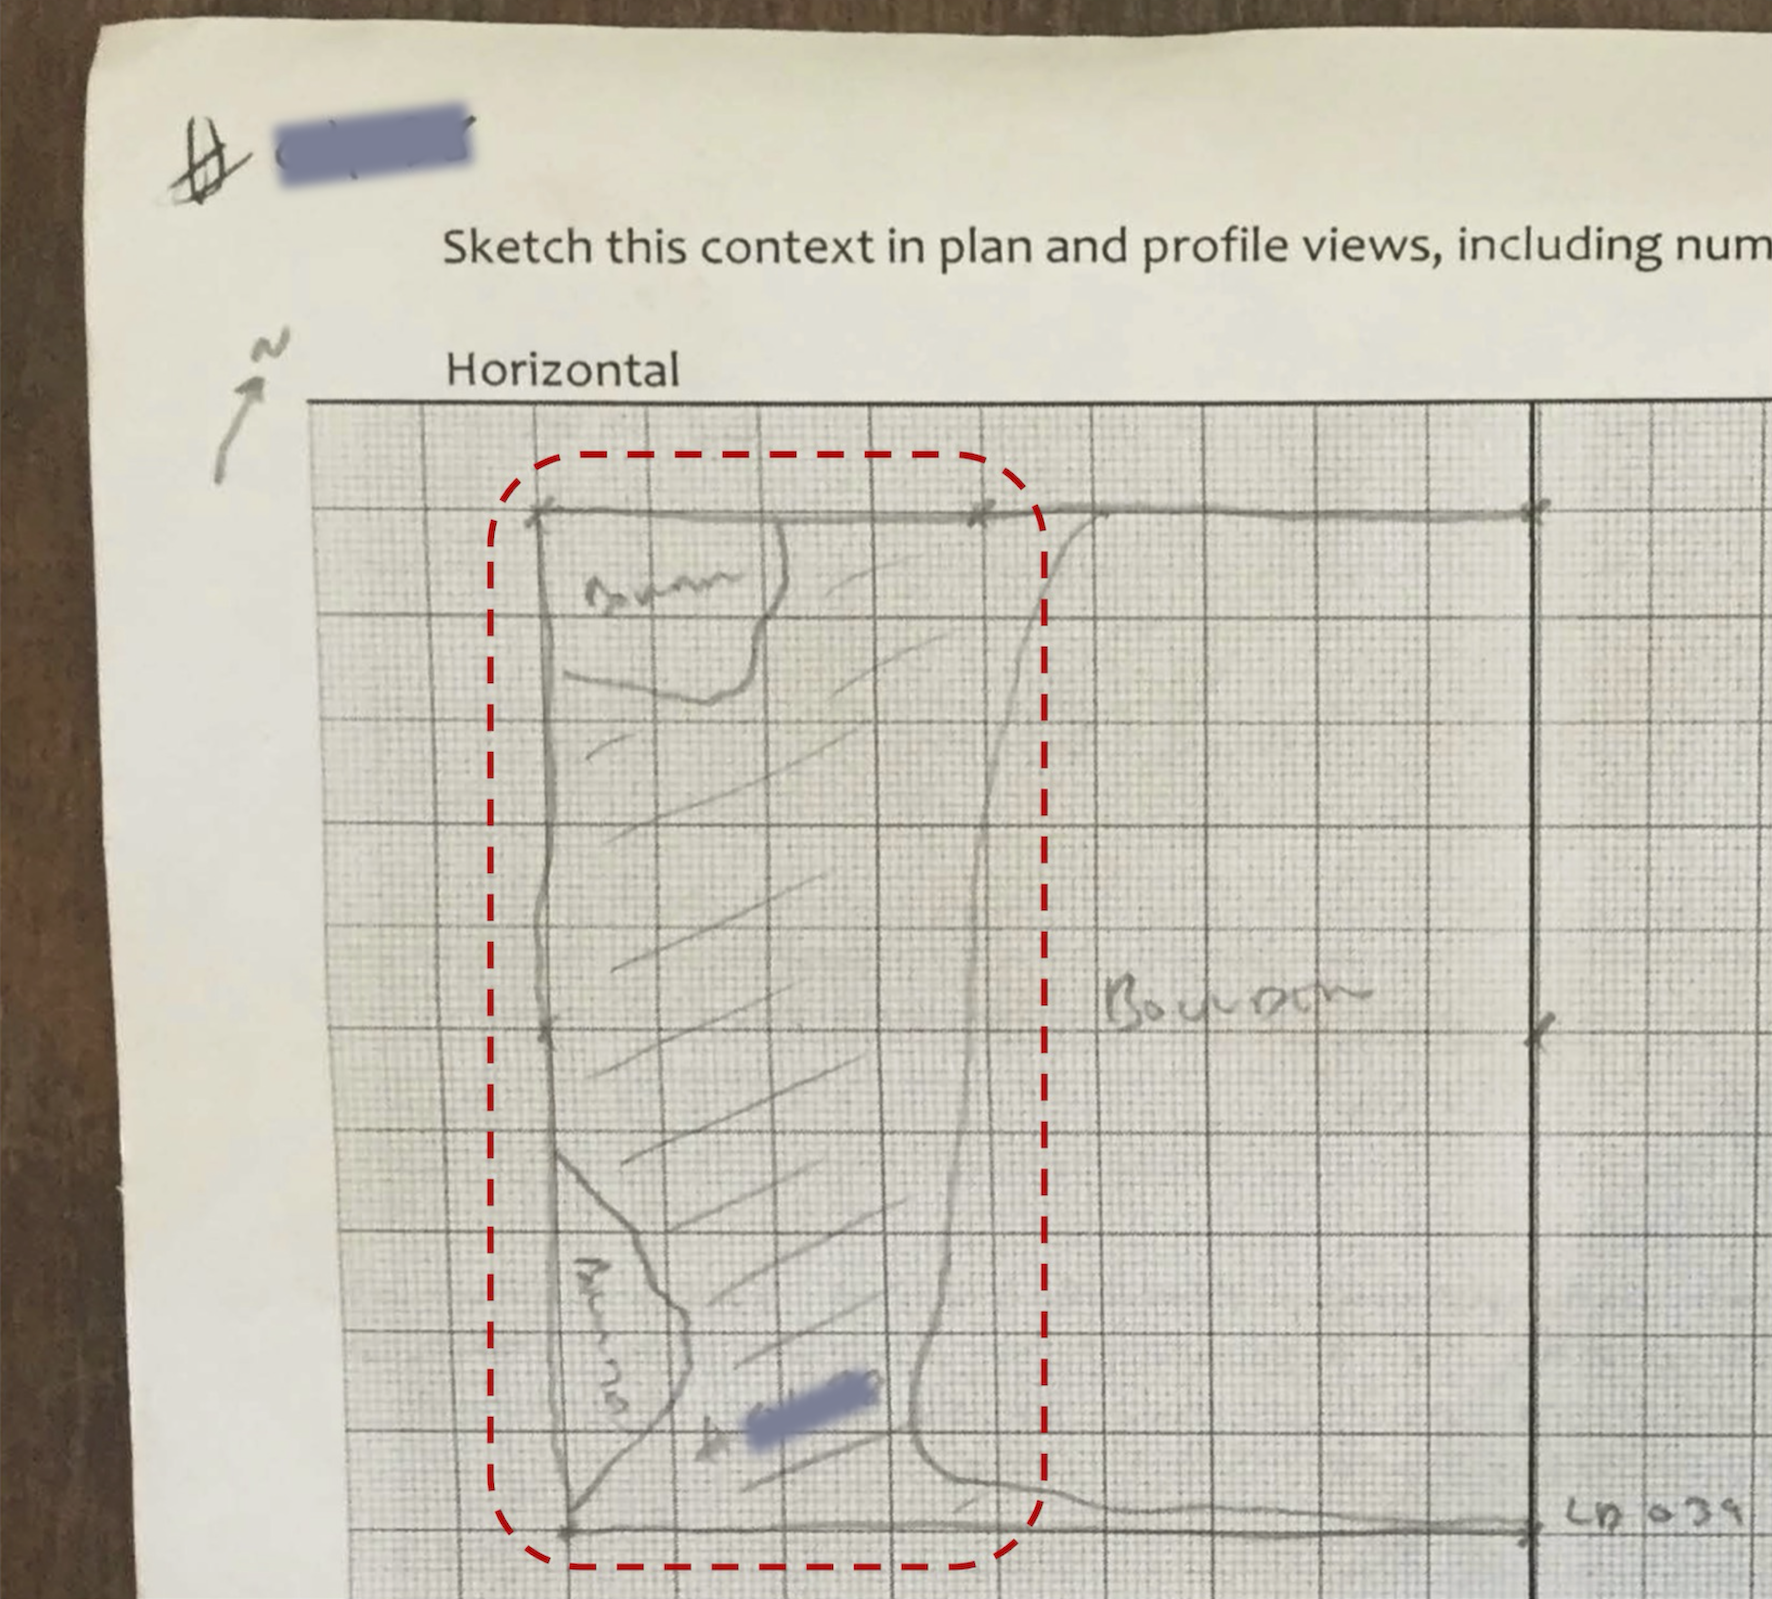
\includegraphics[keepaspectratio]{figures/context-sketch.png}}

}

\caption{\label{fig-context-sketch}Sketch of the base of a trench,
portraying the context addressed in the observed episode, boxed in red.}

\end{figure}%

\begin{figure}

\centering{

\pandocbounded{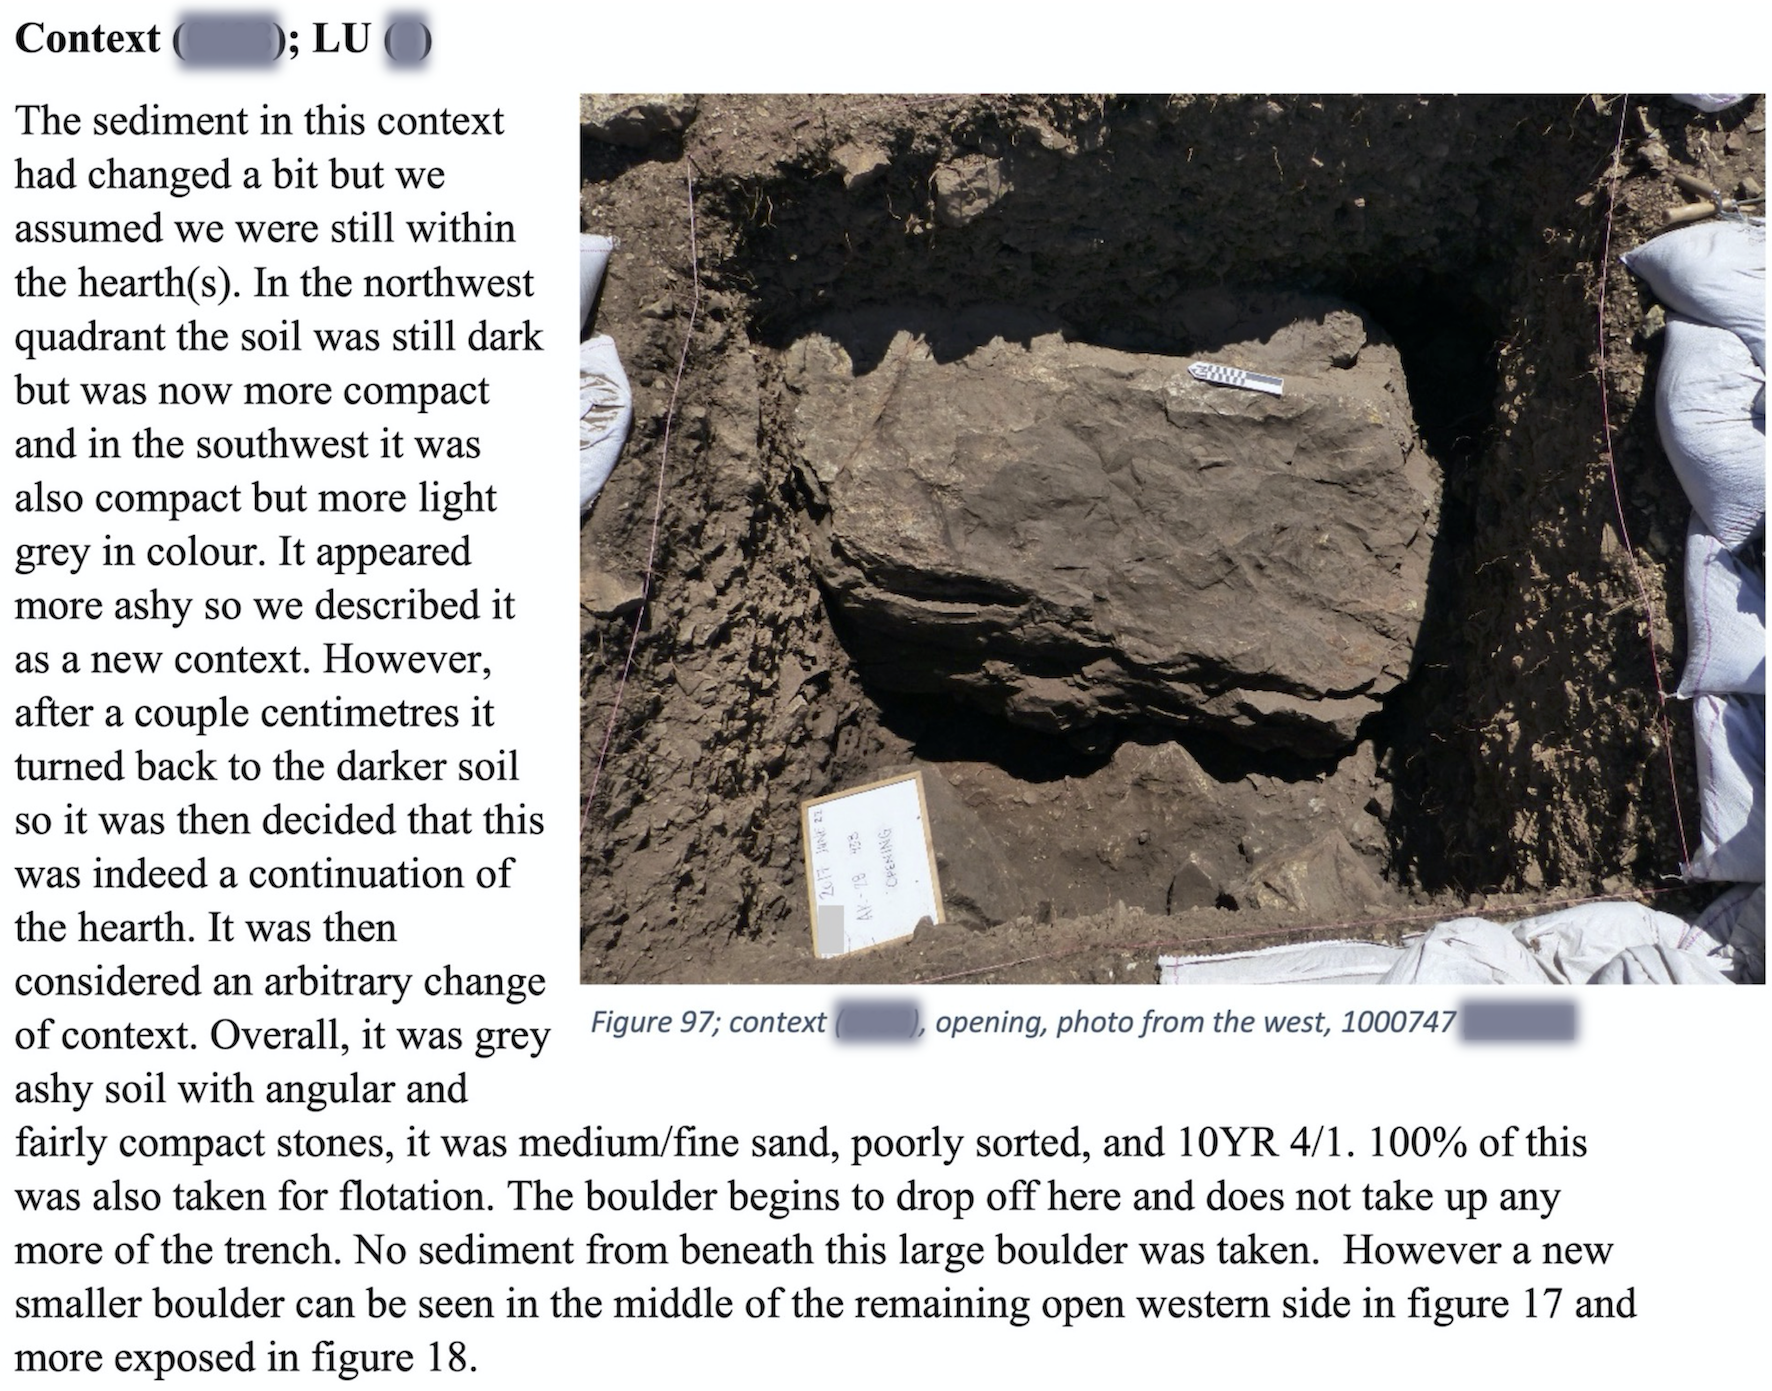
\includegraphics[keepaspectratio]{figures/context-report.png}}

}

\caption{\label{fig-context-report}Section of a trench report describing
the context addressed in the observed episode, and situating it as part
of a lithostratigraphic unit.}

\end{figure}%

In particular, the tentativity and ambiguity that Jane and Basil
experienced while excavating this trench was one of its notable
properties, as elicited in the final trench report (see
Figure~\ref{fig-context-report}). Additionally, the report described how
the contexts were eventually lumped together into a more concretely
defined ``lithostratigraphic unit,'' which was formally delimited using
nominal and standardized terminology. In this way, the report switched
back and forth between ambiguous and concrete representations, which
conveyed experiential and distant perspectives, respectively. This
resembles the tone switching that occurred in the conversation between
Jane and Basil, whereby Basil, as supervisor responsible for creating
formal documentation, re-presented Jane's experiences using more formal
terms. As such, this reflects an implicit recognition that there is
immense value in being able to share more nuanced perspectives on the
things that make up the archaeological record. At the same time, and in
contrast with truly situated records like those maintained in field
journals (cf. Batist 2024), the language documenting such tentativity in
the report remained largely impersonal and observations were de-situated
and disembodied.

It is notable that situated experiences were recorded in the
report-writing phase, and only by those acting in authoritative roles.
This parallels how field journals --- which are also records of situated
experiences --- are exclusively maintained by supervising personnel
(Batist 2024). These observations reflect the different kinds of agency
held by different actors in the project. Fieldworkers were encouraged to
shape their behaviour so that the information they obtained was born as
formal entities from the start, whereas those responsible for presenting
the record as part of a broader scope of work were responsible for
re-situating the data as products of data-collection processes that they
designed and dictated. Recognizing the situatedness of data while they
were being collected would have warranted recognition of their
limitations, which fieldworkers believed would enable undisciplined data
collection behaviour.\textsuperscript{\hyperref[sec-A20]{A20}}

In other words, the constitution of archaeological records involved
temporarily suspending disbelief regarding the stability of
archaeological observations among fieldworkers, and then re-integration
of storied accounts about the record's origins by supervisors who were
granted greater creative agency. However, this was conditioned through
the use of language that rendered prior work as generic and non-situated
processes, thereby obscuring the agency of those whose work the report
was based on. Although not specifically targeted for this study, similar
tendencies may also be casually observed while re-contextualizing prior
work as part of broader narratives at various scales --- in summaries
about a trench, an area, a site, and even an entire region.

\section{Discussion and Conclusion}\label{discussion-and-conclusion}

This paper's findings demonstrate how the production of stable and
concrete archaeological records involves characterizing the phenomena of
interest in nominal terms, while downplaying the situated and embodied
experiences that informed the records' creation. More specifically, it
documents a tendency toward enforcing formally-defined records in
support of analytical tasks down the line, which present fieldwork as a
means to an end, and fieldworkers as instruments that can be wielded to
support future analytic endeavours. It shows how these values are
instilled through the social and material experiences in which fieldwork
is embedded, which inform fieldworkers about how their labour, and the
outcomes of their labour, contribute to collective efforts. In other
words, it reveals how the management of archaeological data and of
archaeological labour are inherently intertwined, and draws attention to
some mechanisms through which certain voices are rendered more visible
than others when constituting the archaeological record.

Moreover, the fieldworkers I observed and spoke with played into the
roles they were assigned, even though this meant having less creative
agency. In fact, they generally valued their contributions as sensory
devices, which is linked to the notion that they were capable of seeing
things as they really are --- as material entities that have seemingly
not yet been ascribed stable meaning. As such, fieldworkers actively
contributed to honing the illusion of their objectivity, which enhanced
their value as members of the project and as domain specialists with
their own unique mental skills. At the same time, it was also clear that
fieldworkers knew, on an intuitive level, that any claim of objectivity
is overstated (as per complementary work published in Batist 2024: 12).
However, their positions as responsive rather than creative actors
ensured that they are not responsible for resolving this tension (cf.
Batist, In review).

These findings complement other empirical research examining
archaeological data management as collective interpretive action. For
instance, Batist et al. (2021) and Batist (In review) note that rote
fieldwork practices tend to be assigned to relatively junior project
personnel, who become ensnared in workflows which discipline their
actions. Similarly, Morgan and Wright (2018), who compare analog and
digital field drawing techniques, reveal how the act of transcribing
archaeological deposits on a blank surface produces greater
understanding in the minds of students than participating as a cog in a
broader digital apparatus, owing to different degrees of creative
interpretive agency that each method affords them. Moreover, Yarrow
(2008), who examines the meaning, materiality and agency in
archaeological recording practices, draws attention to expressions of
resignation among fieldworkers who were more aware that the information
they record does not hold special meaning, based on their prior
understanding of how these records would actually be used down the line.
Thorpe (2012), Zorzin (2010), Edgeworth (1991) and Watson (2019)
highlight similar perspectives in their critical investigations of
agentic relationships and knowledge production in commercial
archaeology.

This paper has clear implications for thinking about data documentation
and the potential for data to be re-used in secondary research contexts,
at greater distance from their contexts of creation. Surveys and
experiments by Faniel et al. (2013: 299-301), Atici et al. (2013:
676-677), Kansa and Whitcher Kansa (2013: 90-91) and Chapman and Wylie
(2016: 213), which investigated the needs of data re-users, highlighted
their desires to communicate directly with datasets' creators to
ascertain the subtext hidden between the lines of their formal
documentation. This aligns with investigations of attempts to enhance
archaeological documentation by Huvila, Börjesson, and Sköld (2022),
Austin et al. (2024) and Opitz et al. (2021), which suggest that such
efforts should be directed by specific contexts of re-use. A common
thread across these investigations on either end of the archive is that
effective data-sharing must involve some discursive relationship between
those who produce and re-use data, thereby bridging the epistemic
distance imposed by layers of abstraction (Huggett 2022b). Strategies
for enhancing data's re-use potential across the continuum of
archaeological practice thereby embody Dallas' (2015) notion of curation
as simultaneous acts of reconciliation and anticipation, whereby
meanings are negotiated in relation to prior and future objectives and
circumstances.

However, the systemic drive to produce certain kinds of information
outcomes based on confident and stable data sources is not fully
compatible with this need to acknowledge the complex and storied
histories of data. This tension between distinct notions of data, as
concrete and disembodied records in one sense, and as situated products
of decisions, actions and circumstances in another, produces an
epistemic anxiety that archaeologists must cope with. It is unclear how,
or even if, this epistemic tension can be resolved, but the drive to
achieve a state of objectivity in fieldwork, which is facilitated by
systemic distributions of agency, persists --- in spite of this
outcome's impossibility --- as one coping mechanism.

To be clear, the instrumentalisation of archaeological labour is often
necessary in order to derive concrete and confident records that are
suitable for analytical methods which comply with modern scientific
quality standards. Moreover, information commons, such as the pool of
knowledge accumulated throughout an archaeological project, do not
necessarily have to be egalitarian, and are always governed by norms and
expectations concerning who may contribute to and extract from communal
resources, and in what ways these interactions should occur. But rather
than lean in to the illusion of archaeological objectivity, which is a
value built in to most contemporary data management systems, it may be
prudent to try an alternative approach that fosters a commensal attitude
toward data; namely, one which more fully recognizes data work occurring
throughout the continuum of archaeological practice, including in
domains that are not typically recognized for their capacity to work
with data, such as fieldwork.

\newpage

\section{References}\label{references}

\phantomsection\label{refs}
\begin{CSLReferences}{1}{0}
\bibitem[\citeproctext]{ref-atici2013}
Atici, Levent, Sarah Whitcher Kansa, Justin Lev-Tov, and Eric C. Kansa.
2013. {``Other {People}'s {Data}: {A Demonstration} of the {Imperative}
of {Publishing Primary Data}.''} \emph{Journal of Archaeological Method
and Theory} 20 (4): 663.
\url{https://doi.org/10.1007/s10816-012-9132-9}.

\bibitem[\citeproctext]{ref-austin2024}
Austin, Anne, Ixchel M. Faniel, Brittany Brannon, and Sarah Whitcher
Kansa. 2024. {``Improving the {Usability} of {Archaeological Data}
Through {Written Guidelines}.''} \emph{Advances in Archaeological
Practice}, January, 1--12. \url{https://doi.org/10.1017/aap.2023.38}.

\bibitem[\citeproctext]{ref-batist-alienation}
Batist, Zachary. In review. {``Locating Creative Agency in
Archaeological Data Work.''} \emph{Peer Community In Archaeology}.
\url{https://doi.org/10.17613/8eqy4-n1m82}.

\bibitem[\citeproctext]{ref-batist2023a}
---------. 2023. {``Archaeological Data Work as Continuous and
Collaborative Practice.''} PhD thesis, Toronto: University of Toronto.
\url{https://hdl.handle.net/1807/130306}.

\bibitem[\citeproctext]{ref-batist2024a}
---------. 2024. {``On the {Value} of {Informal Communication} in
{Archaeological Data Work}.''} \emph{Open Archaeology} 10 (1): 20240014.
\url{https://doi.org/10.1515/opar-2024-0014}.

\bibitem[\citeproctext]{ref-batist2021}
Batist, Zachary, Val Masters, Tiffany C. Torma, Michael Carter, Neal
Ferris, Isto Huvila, Seamus Ross, and Costis Dallas. 2021.
{``Figurations of {Digital Practice}, {Craft}, and {Agency} in {Two
Mediterranean Fieldwork Projects}.''} \emph{Open Archaeology} 7 (1):
1731--55. \url{https://doi.org/10.1515/opar-2020-0217}.

\bibitem[\citeproctext]{ref-berggren2012}
Berggren, Åsa. 2012. {``Comments on {Matt Edgeworth}: {`{Follow} the
{Cut}, {Follow} the {Rhythm}, {Follow} the {Material}'}.''}
\emph{Norwegian Archaeological Review} 45 (1): 92--94.
\url{https://doi.org/10.1080/00293652.2012.679425}.

\bibitem[\citeproctext]{ref-berggren2015}
Berggren, Åsa, Nicolo Dell'Unto, Maurizio Forte, Scott Haddow, Ian
Hodder, Justine Issavi, Nicola Lercari, Camilla Mazzucato, Allison
Mickel, and James S. Taylor. 2015. {``Revisiting Reflexive Archaeology
at {Çatalhöyük}: {Integrating} Digital and {3D} Technologies at the
Trowel's Edge.''} \emph{Antiquity} 89 (344): 433--48.
\url{https://doi.org/10.15184/aqy.2014.43}.

\bibitem[\citeproctext]{ref-bevan2012a}
Bevan, Andrew. 2012. {``Value, {Authority} and the {Open Society}. {Some
Implications} for {Digital} and {Online Archaeology}.''} In
\emph{Archaeology and {Digital Communication}: {Towards Strategies} of
{Public Engagement}}, edited by Chiara Bonacchi, 1--14. London, UK:
Archetype.

\bibitem[\citeproctext]{ref-bowen2006}
Bowen, Glenn A. 2006. {``Grounded {Theory} and {Sensitizing
Concepts}:''} \emph{International Journal of Qualitative Methods} 5 (3):
12--23. \url{https://doi.org/10.1177/160940690600500304}.

\bibitem[\citeproctext]{ref-caraher2019}
Caraher, William. 2019. {``Slow {Archaeology}, {Punk Archaeology}, and
the {`{Archaeology} of {Care}'}.''} \emph{European Journal of
Archaeology} 22 (3): 372--85. \url{https://doi.org/10.1017/eaa.2019.15}.

\bibitem[\citeproctext]{ref-chadwick1998}
Chadwick, Adrian. 1998. {``Archaeology at the Edge of Chaos: Further
Towards Reflexive Excavation Methodologies.''} \emph{Assemblage}
3:97--117.

\bibitem[\citeproctext]{ref-chapman2016}
Chapman, Robert, and Alison Wylie. 2016. \emph{Evidential {Reasoning} in
{Archaeology}}. Bloomsbury Academic.
\url{https://books.google.com?id=tMohDQAAQBAJ}.

\bibitem[\citeproctext]{ref-charmaz2000}
Charmaz, Kathy. 2000. {``Grounded {Theory}: {Objectivist} and
{Constructionist Methods}.''} In \emph{Handbook of {Qualitative
Research}}, edited by Norman K. Denzin and Yvonna S. Lincoln, 2nd ed.,
509--36. Thousand Oaks, CA: SAGE.

\bibitem[\citeproctext]{ref-charmaz2014}
---------. 2014. \emph{Constructing {Grounded Theory}}. 2nd ed. SAGE.

\bibitem[\citeproctext]{ref-dallas2015}
Dallas, Costis. 2015. {``Curating {Archaeological Knowledge} in the
{Digital Continuum}: {From Practice} to {Infrastructure}.''} \emph{Open
Archaeology} 1 (1): 176--207.
\url{https://doi.org/10.1515/opar-2015-0011}.

\bibitem[\citeproctext]{ref-edgeworth1991}
Edgeworth, Matt. 1991. {``The Act of Discovery: {An} Ethnography of the
Subject-Object Relation in Archaeological Practice.''} PhD thesis,
Durham University. \url{http://etheses.dur.ac.uk/1481/}.

\bibitem[\citeproctext]{ref-edgeworth2003}
---------. 2003. \emph{Acts of Discovery: {An} Ethnography of
Archaeological Practice}. Vol. 1131. British Archaeological Reports.

\bibitem[\citeproctext]{ref-everill2007}
Everill, Paul. 2007. {``A {Day} in the {Life} of a {Training
Excavation}: {Teaching Archaeological Fieldwork} in the {UK}.''}
\emph{World Archaeology} 39 (4): 483--98.
\url{https://doi.org/10.1080/00438240701676243}.

\bibitem[\citeproctext]{ref-faniel2013}
Faniel, Ixchel, Eric C. Kansa, Sarah Whitcher Kansa, Julianna
Barrera-Gomez, and Elizabeth Yakel. 2013. {``The {Challenges} of
{Digging Data}: {A Study} of {Context} in {Archaeological Data
Reuse}.''} In \emph{Proceedings of the 13th {ACM}/{IEEE-CS Joint
Conference} on {Digital Libraries}}, 295--304. New York: ACM.
\url{https://doi.org/10.1145/2467696.2467712}.

\bibitem[\citeproctext]{ref-flick1997}
Flick, Uwe. 1997. {``The Episodic Interview. {Small} Scale Narratives as
Approach to Relevant Experiences.''} \emph{London School of Economics
Methodology Institute: Discussion Papers-Qualitative Series}.

\bibitem[\citeproctext]{ref-flick2000}
---------. 2000. {``Episodic {Interviewing}.''} In \emph{Qualitative
{Researching} with {Text}, {Image} and {Sound}}, by Martin Bauer and
George Gaskell, 76--92. London: SAGE Publications Ltd.
\url{https://doi.org/10.4135/9781849209731.n5}.

\bibitem[\citeproctext]{ref-gero1994}
Gero, Joan M. 1994. {``Excavation {Bias} and the {Woman} at {Home
Ideology}.''} \emph{Archeological Papers of the American Anthropological
Association} 5 (1): 37--42.
\url{https://doi.org/10.1525/ap3a.1994.5.1.37}.

\bibitem[\citeproctext]{ref-gero1996}
---------. 1996. {``Archaeological Practice and Gendered Encounters with
Field Data.''} \emph{Gender and Archaeology}, 251--80.

\bibitem[\citeproctext]{ref-goodwin1994}
Goodwin, Charles. 1994. {``Professional {Vision}.''} \emph{American
Anthropologist} 96 (3): 606--33.
\url{https://doi.org/10.1525/aa.1994.96.3.02a00100}.

\bibitem[\citeproctext]{ref-goodwin2010}
---------. 2010. {``Things and Their Embodied Environments.''} In
\emph{The Cognitive Life of Things: {Recasting} the Boundaries of the
Mind}, edited by Lambros Malafouris and Colin Renfrew, 103--20.
Cambridge: McDonald Institute of Archaeological Research.

\bibitem[\citeproctext]{ref-graham2019}
Graham, Shawn. 2019. \emph{Failing Gloriously and Other Essays}. Grand
Forks, North Dakota: The Digital Press at the University of North
Dakota. \url{https://doi.org/10.31356/dpb015}.

\bibitem[\citeproctext]{ref-haciguzeller2021}
Hacıgüzeller, Piraye, James Stuart Taylor, and Sara Perry. 2021. {``On
the {Emerging Supremacy} of {Structured Digital Data} in {Archaeology}:
{A Preliminary Assessment} of {Information}, {Knowledge} and {Wisdom
Left Behind}.''} \emph{Open Archaeology} 7 (1): 1709--30.
\url{https://doi.org/10.1515/opar-2020-0220}.

\bibitem[\citeproctext]{ref-huggett2022}
Huggett, Jeremy. 2022a. {``Data {Legacies}, {Epistemic Anxieties}, and
{Digital Imaginaries} in {Archaeology}.''} \emph{Digital} 2 (2):
267--95. \url{https://doi.org/10.3390/digital2020016}.

\bibitem[\citeproctext]{ref-huggett2022a}
---------. 2022b. {``Is {Less More}? {Slow Data} and {Datafication} in
{Archaeology}.''} In \emph{Critical {Archaeology} in the {Digital Age}:
{Proceedings} of the 12th {IEMA Visiting Scholar}'s {Conference}},
edited by Kevin Garstki, 97--110. Los Angeles, CA: Cotsen Institute of
Archaeology Press.
\url{https://escholarship.org/uc/item/0vh9t9jq\#page=112}.

\bibitem[\citeproctext]{ref-huvila2011}
Huvila, Isto. 2011. {``Being Formal and Flexible: Semantic Wiki as an
Archaeological e-Science Infrastructure.''} In \emph{Revive the {Past}:
{Proceeding} of the 39th {Conference} on {Computer Applications} and
{Quantitative Methods} in {Archaeology}, {Beijing}}, 186--97.

\bibitem[\citeproctext]{ref-huvila2016}
---------. 2016. {``"{If We Just Knew Who Should Do It}", or the {Social
Organization} of the {Archiving} of {Archaeology} in {Sweden}.''}
\emph{Information Research: An International Electronic Journal} 21 (2):
n2. \url{https://eric.ed.gov/?id=EJ1104372}.

\bibitem[\citeproctext]{ref-huvila2022b}
Huvila, Isto, Lisa Börjesson, and Olle Sköld. 2022. {``Archaeological
Information-Making Activities According to Field Reports.''}
\emph{Library \& Information Science Research} 44 (3): 101171.
\url{https://doi.org/10.1016/j.lisr.2022.101171}.

\bibitem[\citeproctext]{ref-kansa2013}
Kansa, Eric C., and Sarah Whitcher Kansa. 2013. {``We {All Know That} a
14 {Is} a {Sheep}: {Data Publication} and {Professionalism} in
{Archaeological Communication}.''} \emph{Journal of Eastern
Mediterranean Archaeology and Heritage Studies} 1 (1): 88--97.
\url{https://doi.org/10.1353/ema.2013.0007}.

\bibitem[\citeproctext]{ref-lucas2019}
Lucas, Gavin. 2019. \emph{Writing the Past: {Knowledge} and Literary
Production in Archaeology}. Abingdon, Oxon ; New York, NY: Routledge.

\bibitem[\citeproctext]{ref-mickel2021}
Mickel, Allison. 2021. \emph{Why {Those Who Shovel Are Silent}: {A
History} of {Local Archaeological Knowledge} and {Labor}}. University
Press of Colorado. \url{https://doi.org/10.5876/9781646421152}.

\bibitem[\citeproctext]{ref-morgan2018}
Morgan, Colleen, and Holly Wright. 2018. {``Pencils and {Pixels}:
{Drawing} and {Digital Media} in {Archaeological Field Recording}.''}
\emph{Journal of Field Archaeology} 43 (2): 136--51.
\url{https://doi.org/10.1080/00934690.2018.1428488}.

\bibitem[\citeproctext]{ref-morse2019}
Morse, Janice M., and Lauren Clark. 2019. {``The {Nuances} of {Grounded
Theory Sampling} and the {Pivotal Role} of {Theoretical Sampling}.''} In
\emph{The {SAGE Handbook} of {Current Developments} in {Grounded
Theory}}, by Antony Bryant and Kathy Charmaz, 145--66. 1 Oliver's
Yard,~55 City Road~London~EC1Y 1SP: SAGE Publications Ltd.
\url{https://doi.org/10.4135/9781526436061.n9}.

\bibitem[\citeproctext]{ref-opitz2021}
Opitz, Rachel, Colleen Strawhacker, Philip Buckland, Jackson Cothren,
Tom Dawson, Andrew Dugmore, George Hambrecht, et al. 2021. {``A
{Lockpick}'s {Guide} to {dataARC}: {Designing Infrastructures} and
{Building Communities} to {Enable Transdisciplinary Research}.''}
\emph{Internet Archaeology} 56 (October).
\url{https://doi.org/10.11141/ia.56.15}.

\bibitem[\citeproctext]{ref-ragin1992}
Ragin, Charles C. 1992. {``Casing and the Process of Social Research.''}
In \emph{What Is a {Case}? {Exploring} the {Foundations} of {Social
Inquiry}}, edited by Charles C. Ragin and Howard S. Becker, 217--26.
Cambridge University Press New York.

\bibitem[\citeproctext]{ref-thorpe2012}
Thorpe, Reuben. 2012. {``Often {Fun}, {Usually Messy}: {Fieldwork},
{Recording} and {Higher Orders} of {Things}.''} In \emph{Reconsidering
{Archaeological Fieldwork}: {Exploring On-Site Relationships Between
Theory} and {Practice}}, edited by Hannah Cobb, Harris Harris Oliver J.
T., Cara Jones, and Philip Richardson, 31--52. Springer, Boston, MA.
\url{https://doi.org/10.1007/978-1-4614-2338-6_3}.

\bibitem[\citeproctext]{ref-voss2012}
Voss, Barbara L. 2012. {``Curation as Research. {A} Case Study in
Orphaned and Underreported Archaeological Collections.''}
\emph{Archaeological Dialogues} 19 (2): 145--69.
\url{https://doi.org/10.1017/s1380203812000219}.

\bibitem[\citeproctext]{ref-watson2019}
Watson, Sadie. 2019. {``Whither Archaeologists? {Continuing} Challenges
to Field Practice.''} \emph{Antiquity} 93 (372): 1643--52.
\url{https://doi.org/10.15184/aqy.2019.141}.

\bibitem[\citeproctext]{ref-witzel2000}
Witzel, Andreas. 2000. {``The Problem-Centered Interview.''} \emph{Forum
Qualitative Sozialforschung / Forum: Qualitative Social Research} 1 (1).
\url{https://doi.org/10.17169/fqs-1.1.1132}.

\bibitem[\citeproctext]{ref-wylie2017}
Wylie, Alison. 2017. {``How {Archaeological Evidence Bites Back}:
{Strategies} for {Putting Old Data} to {Work} in {New Ways}.''}
\emph{Science, Technology, \& Human Values} 42 (2): 203--25.
\url{https://doi.org/10.1177/0162243916671200}.

\bibitem[\citeproctext]{ref-yarrow2008}
Yarrow, Thomas. 2008. {``In {Context}: {Meaning}, {Materiality} and
{Agency} in the {Process} of {Archaeological Recording}.''} In
\emph{Material {Agency}: {Towards} a {Non-Anthropocentric Approach}},
edited by Carl Knappett and Lambros Malafouris, 121--37. Boston, MA:
Springer. \url{https://doi.org/10.1007/978-0-387-74711-8_7}.

\bibitem[\citeproctext]{ref-zorzin2010}
Zorzin, Nicolas. 2010. {``The Political Economy of a Commercial
Archaeology a {Quebec} Case-Study.''} University of Southampton.
\url{https://eprints.soton.ac.uk/344777/}.

\bibitem[\citeproctext]{ref-zorzin2015}
---------. 2015. {``Dystopian {Archaeologies}: {The Implementation} of
the {Logic} of {Capital} in {Heritage Management}.''}
\emph{International Journal of Historical Archaeology} 19 (4): 791--809.
\url{https://doi.org/10.1007/s10761-015-0315-4}.

\end{CSLReferences}

\newpage

\subsection{Acknowledgments}\label{acknowledgments}

I extend warm thanks to Costis Dallas, Matt Ratto, Ted Banning, Jeremy
Huggett and Ed Swenson for supervising my work and providing critical
feedback as I conducted my doctoral research, which this paper is based
upon. I am also very grateful to the anonymous reviewers for their
constructive evaluation. Of course, this work would not have been
possible without the anonymous research participants who allowed me to
observe and interview them as they worked, and to articulate their
actions and outlooks.

Permits were not required for this research.

\subsection{Funding}\label{funding}

This work is derived from the author's doctoral dissertation,
\emph{Archaeological data work as continuous and collaborative practice}
(Batist 2023), which was supported by the Canadian Social Sciences and
Humanities Research Council Doctoral Fellowship (Award ID:
752-2019-2233).

\subsection{Competing Interests}\label{competing-interests}

The author states no conflicts of interest.

\subsection{Author Contribution}\label{author-contribution}

Zachary Batist is the sole author of this work. He defined the scope of
the study and identified suitable cases for inclusion, collected and
processed all data, performed analysis, interpreted the findings,
created all the figures, and wrote the paper.

\subsection{Informed Consent}\label{informed-consent}

Informed consent has been obtained from all individuals included in this
study, in compliance with the University of Toronto's Social Sciences,
Humanities, and Education Research Ethics Board, Protocol 34526.

\subsection{Data Availability
Statement}\label{data-availability-statement}

The data generated and analyzed during the current study are included in
this published article's supplementary files.

\subsection{Author Bio}\label{author-bio}

Zachary Batist obtained his PhD from the University of Toronto's Faculty
of Information. His research explores the collaborative commitments
inherent throughout archaeological practice, especially relating to data
management and the constitution of information commons. He currently
works as a Postdoctoral Researcher at the Department of Epidemiology,
Biostatistics and Occupational Health in the School of Population and
Global Health at McGill University, where he investigates the
collaborative, technical and administrative structures that scaffold
data harmonization in epidemiological research.

\newpage

\section{Supplementary Materials}\label{supplementary-materials}

These supplementary materials include a summary of the participants'
backgrounds and extracts of specific observations and interviews
referenced throughout the paper.

\subsection{Summary of Participants' Roles and
Backgrounds}\label{summary-of-participants-roles-and-backgrounds}

Here is a list and brief description of individuals mentioned throughout
the paper:

\textbf{Basil:} Project director and faculty member at a North American
university. He has extensive field experience and has consulted as a
lithics specialist for various other projects, where he met many of the
people who became involved with the project that he now leads.

\textbf{Jane:} One of Basil's top students, who joined the project for
one season. As a very independent and competent worker, she took on
supervisory responsibilities and stood out as an exemplary fieldworker.

\textbf{Theo:} Commercial archaeologist, recommended to Basil by a
mutual friend. An excavator by profession, his competence often serves
as an example for the rest of the crew. He became field director after a
few years working as a trench supervisor. He is very laid back and has a
casual attitude.

\textbf{Ben:} One of Basil's top students, who joined as a trench
assistant. He came back the following year as a trench supervisor.

\textbf{Alfred:} Senior graduate student working at the project for his
geoarchaeology dissertation at a North American university. At a certain
point he took on the role of field director. He is confident, with a
hands-on, get-things-done attitude.

\begin{center}\rule{0.5\linewidth}{0.5pt}\end{center}

Here is a list and brief description of individuals mentioned throughout
the referenced materials but who do not appear in the main section of
the paper:

\textbf{Dorothy:} Senior graduate student who oversees palaeobotanical
analysis, including sample collection and processing protocols.

\textbf{Jolene:} Senior graduate student who oversees the analysis of
chipped stone for the project. She met Basil while working at another
project.

\textbf{Agatha:} Graduate student who serves as Jolene's assistant. Her
specialty is ground-stone artefacts but in this project she largely
performs logistical duties.

\textbf{Talia:} Junior faculty member who became involved with the
project as a trench supervisor after a colleague recommended her to
Basil.

\textbf{Lauren:} Graduate student who became involved with the project
as a trench supervisor after a colleague recommended her to Basil.

\textbf{Lester:} Commercial archaeologist who became involved with the
project as a trench supervisor after Theo recommended him to Basil.

\textbf{Olivia:} Commercial archaeologist who became involved with the
project as a trench supervisor after Alfred recommended her to Basil.

\subsection{Observations and
Elicitations}\label{observations-and-elicitations}

\subparagraph{A1}\label{sec-A1}

\textbf{Jane:} Approaching another context, I think.\\
\textbf{Zack:} Why do you think that?\\
\textbf{Jane:} The texture is changing, and the colour is changing a
bit, and umm, there's a layer of big boulders and now there isn't.\\
\textbf{Zack:} Can you be more specific?\\
\textbf{Jane:} Well the darker sand is becoming more red, which is
similar to what we had there, and then I also noticed that is holds more
of a form, like the hearth is very loose, but the sand is more in place,
it's almost like if you brushed it, you would get a perfect floor.

\subparagraph{A2}\label{sec-A2}

\textbf{Jane:} So, this is like still kind of a dark, dark brown, going
into the sand, but it's like really tough, like hard to dig through,
kind of. So I think maybe it's just context {[}?{]}. ((gesturing towards
other side of the trench)) And then this is like really light grey,
((bobs hand up and down to emphasize these last three words)) and I
thought it was just cuz it had just dried out, and I hadn't done this
kind of {[}fill{]}, but it's also really hard to dig, and like a really
light grey, so I don't know if it's just remnants of this part, or
what...\\
((Basil gets in the trench to take a closer look))\\
\textbf{Jane:} Or like maybe this is like, would it be possible that
that's like an older hearth, like the other one that was leached out?\\
\textbf{Basil:} Yeah, hmm. So the colour here is the same as what you
were digging, but the consistency has changed?\\
\textbf{Jane:} Yeah\\
\textbf{Basil:} I would clean up, maybe just straighten that section a
bit\\
\textbf{Jane:} Yeah\\
\textbf{Basil:} Just to the depth that you started at for this context\\
\textbf{Jane:} Yeah\\
\textbf{Basil:} And then we'll clean up and carry on with, you know, we
can just write in the text that, you know, these are the differences\\
\textbf{Jane:} Yeah\\
\textbf{Basil:} But you know what, after we start to dig it it might
change back to something more familiar\\
\textbf{Jane:} Yeah\\
\textbf{Basil:} And we can just say oh, it's like some kind of
differential lens of material within it\\
\textbf{Jane:} Right\\
\textbf{Jane:} Okay. Okay, so just clean up the walls, and then keep
going, okay.\\
\textbf{Basil:} Yeah, but we can photograph, change numbers.\\
\textbf{Jane:} Oh, okay.\\
\textbf{Basil:} We'll treat it as something different, you know we can
write in the notes that there is a very good chance that it's still the
same stuff, but the consistency changed\\
\textbf{Jane:} Right.\\
\textbf{Basil:} So, just be careful.

\subparagraph{A3}\label{sec-A3}

\textbf{Zack:} Did you feel like there are, like, problems, with
communicating, in terms of like understanding, sort of the things that
like Alfred was getting at? Or like, if there were any issues in like,
uhh, comprehending something that eventually you sort of learned, or
were there any sort of challenges in that sense that you had to deal
with? Do you recall any examples like that? Especially maybe in the
beginning.\\
\textbf{Jane:} I think for a geology it's best, especially like if you
do a couple of geology courses, it's always hard to like train your eyes
to see certain things. Like sometimes Alfred would like take out a
handful of sand and go like do you see the red flakes? and I would be
like no. Or even like, pointing our stratigraphy, like see how this
changes to this level, and it just kind of, training your eye to see
what they're seeing is, sounds like an easy thing but it's actually hard
to like, kind of, pick out things that they want you to pick out. And I
think like now it's easier to like, oh, see how that's transitioning, or
like, umm, even just like comparing peoples' trenches and like the
contexts they're in, it's easier now but at the start it was like, it
looks the same to me, or like I don't spot what you're spotting, you
know? And it's just a way of looking at things that I think that's the
hardest part for me.\\
\textbf{Zack:} Do you know how that developed?\\
\textbf{Jane:} I think just like repetitive, like every day, looking at
stuff, I think is like, just a good way of learning. I don't know if
there's something specific but... and just hearing from like, hearing
Alfred pointing it out, hearing Basil pointing it out, hearing different
supervisors pointing it out, it was just different ways of explaining it
or showing it to you that it starts to kind of, like, produce a form of
knowledge. Umm, but I dunno.

\subparagraph{A4}\label{sec-A4}

\textbf{Lester:} And that was the time I really kind of got into
excavation as a concept. So I did that on my first year. In my second
year, I {[}unclear{]} community archaeology, and then {[}redacted{]}
field school. {[}redacted{]} field school is a big part of
{[}redacted{]} University's training program for their students. I
didn't receive enough excavation experience in my own degree, so I went
and applied and volunteered on that excavation, and then my third year I
went back to the same excavation at a supervisor grade.

\subparagraph{A5}\label{sec-A5}

Had a brief convo with Olivia as she was cleaning up, when the corner
cam died. I really {[}.\ldots{]} by the mic. It was about focus,
{[}awareness?{]} of one's surroundings, being in the moment and focusing
on the task at hand. Focusing on the little things helps her keep her
organized. It is an active strategy in use. She hates that although
excavation is manual labour, it really requires you to actively think.
You can't just phase out -- {[}illegible sentence{]}. I mentioned my
tendency to compare excavation with tunnel vision, and noted how I think
it is somewhat flawed. She asked me if I played a musical instrument,
and I said no, and then asked if I could relate to that. She compared
these activities in order to convey the sense of being in the moment,
facing a task at hand, dealing with what is immediately in front of you,
literally and figuratively, and the satisfaction of achieving one's
goals and ticking off all the boxes. She likes to set goals, for herself
and for others.

\subparagraph{A6}\label{sec-A6}

\textbf{Lester:} So, our first week was tough. Very, very tough. We had
a very uhh difficult trench to excavate, very hard layers that were very
difficult to physically excavate. Uhm and I can dig for a certain
extent, for a period of time in quite hot weather, I'm used to this, for
this is not a problem. But I see people that have never approached this,
attack it physically, really really attack it physically, and not bear
in mind that this is actually really difficult. And it's not a
physicality thing, it's a, it's a thought process. So it's uhh, yes
you're physically able to excavate twenty centimeters in a day, but how
are you going to feel at the end of the day? Are you going to be able to
identify the context while you're doing it? It's better to excavate ten
thoroughly than twenty in a hurry, you know? And, but the speed will
come with time. And so I've noticed this with Morris particularly, he
was quite, he's a very able archaeologist, a very good digger, uhm but
physically he's changed the way he approaches things, so he won't go
full-on that {[}unclear{]} now, and then expect to be able to do it
again the following morning. And then equally, the understanding is
growing, so like contextual change, uhm, I've really struggled to try
and integrate teaching into my methodologies on site, because that's not
my skillset, and not what I'm used to. But now I think we've finally
figured it, I'm involving him in the paperwork a lot more, making that a
part of the teaching process, a bit more. I think it's beneficial.

\subparagraph{A7}\label{sec-A7}

\textbf{Ben:} I think just sometimes, like, I've become too self-aware,
and I get in my head sometimes.\\
\textbf{Zack:} While you're digging?\\
\textbf{Ben:} No, not while I'm digging. Because while I'm digging I'm
like generally busy, and I'm like, like listening to music or whatever

\subparagraph{A8}\label{sec-A8}

\textbf{Zack:} And uhh, the music is a thing, it frames the mood. I'm
trying to think about time and how it frames the day. That's a bit of an
idea that I abandoned and that I want to come back to later on. You
know, sort of, so I need to observe that earlier on in the season, which
I didn't get an opportunity to do.\\
\textbf{Ben:} Yeah. I'll think about that while I'm out there.\\
\textbf{Zack:} How about you?\\
\textbf{Jane:} I'm kind of the same. Like I'd rather just like get going
and like continue going. Like umm, often when Kaitlin is near the trench
and like Basil's not there she'd be like get out, have a break, or like,
Talia likes to be like come out and have a breeze break, but I just
would rather like just keep going until lunch. Like it's just, like
maybe step out once or twice to get water, but like, I find breaking and
like, just kind of like, I like to just start thinking about things and
for me it's just kind of like, get lost in digging and doing your shit,
and then time passes.\\
\textbf{Zack:} Do you get lost digging?\\
\textbf{Jane:} Yeah! I just, like, I started thinking about something
and then I'm... Like it just makes it, like, less of like a, oh when's
gonna be my next break? Or like, even like, that's why I'm kind of glad
we don't talk or like listen to music, because I feel like that would
like frame time more specifically. Whereas like, without any sound it
just kind of like comes, time is like insignificant kinda thing.

\subparagraph{A9}\label{sec-A9}

\textbf{Basil:} I didn't have music in our trenches, and I think I
initially used the excuse that our proximity to umm Gary's house.
Although, of course Gary was only there for the last two weeks. I think
that it might slightly annoy me if I need to be focused, I find it a
distraction. And it's not like it's just in the background. I think, you
know, with Theo and those guys, there's dancing, there's singing along,
which I, if I was right next to them I think it would drive me bananas.
And it probably drove Lauren slightly bananas. Umm, most projects that
I've been on, there hasn't been music. Which, back in the day, you know,
you would need batteries and {[}unclear{]} and what have you, and umm,
so technologically I think it's easier to have music on site now. Umm.
No, but I think there's intimations of it being unprofessional. It's
like, it's it's a distraction from what you're doing. In fact, I worked,
when I worked at Sutton Hoo back in the day, umm, Philip Rahtz, one of
the excavators there, had written a textbook on archaeological field
practice, infamous, umm very old fashioned, and he, he had a famous
section about, umm uhh, during the excavation, the only sound you should
hear is trowel on stone. If you had found something important, you
quietly get up, walk over to the supervisor, bring them over, show them,
you don't {[}unintelligible yelp{]}, you don't make any {[}unclear{]}.
It should be focused and silent. Now I'm not gonna ever go to that
extreme. But uhh, I remember, I think, I mean Alfred, I mean Alfred had
umm, well I mean, it's you know, it's like, office environment. Well,
no, some office environments do have music on. But umm, umm we had uhh,
I think, I mean Alfred had music on in the background. I think he---\\
\textbf{Zack:} Where? In the rock shelter, you mean?\\
\textbf{Basil:} Umm, trench {[}redacted trench ID{]} and when he was
over with Maddie. Umm, he always had music. But it was background music
for him, umm I don't know how loud or whatever, I--- it doesn't appeal
to me. I, I find it a distraction. I can't work here with music. Or if
I'm, if I ever have music on it's because I'm writing emails or I'm
doing something that I can't be distracted by. Umm, sometimes, you know,
I allow myself classical music because it's a foreign language or
there's no lyrics for me to be distracted by. Umm I think Alfred was,
had a problem with, but maybe he didn't see it as his role to umm make
that call, with people being plugged in. So Kaitlin would dig with
headphones in. I think a couple other people might do that as
well.~\textbf{Zack:} I think Jane did too. Don did.\\
\textbf{Basil:} Yeah. Umm. And I think Alfred was like, no, you need to
be more focused on what you're doing. And it was like, I think like, I
didn't feel strongly enough about it, or I felt like the music thing's a
bit weird anyway, that I wasn't gonna come down on people. I might think
about that for, for next time in terms of...

\subparagraph{A10}\label{sec-A10}

\textbf{Zack:} So I have like one more section. We zoomed through this.
I'm wondering about, like, the way you set up, like your research
environments, environment or plural. I mean, do you, I've noticed, but
maybe you don't, maybe you are less able to recognize certain routines
that you get into.\\
\textbf{Lauren:} Oh, totally, totally.\\
\textbf{Zack:} Yeah. And I'm sort of wondering if you could explain any
of those to me.\\
\textbf{Lauren:} Umm, I'm a very organized person. I do need that. So
for me, umm, packing my backpack the same way every morning, knowing
where my things are, sorting stuff out in advance, like taking notes,
for myself, in my own notebook, saying tomorrow you need to do this and
this and this, and knowing where my notebook is, is very important. So I
pack my backpack, either in the evening or in the morning, it doesn't
really matter to me. Umm, I know what material or supplies I need, and
pack them. I bring them and then when we are on site I always put my
backpack in the same place, I take my stuff out in the same, I mean
they're not laid out in order or something, but umm, yeah.

\subparagraph{A11}\label{sec-A11}

\textbf{Zack:} Okay. But with regards to stratigraphy, do you take into
account the other trenches and their stratigraphy? \textbf{Ben:} Oh,
right. Yeah. Because I'm close by to {[}redacted trench ID{]} and a lot
of the reason for opening the trench I'm in now, {[}redacted trench
ID{]}, uhh was to find similar things as {[}redacted trench ID{]}, I am
following, or I am trying to like compare the stratigraphy.

\subparagraph{A12}\label{sec-A12}

\textbf{Lauren:} Exactly. Because I write it down. But still, I enjoy
these interactions with people in my trench. And also people like, we
are, like, in a luxury position on the east side, and we are really
close with our trenches, especially Theo and I, so we can talk about
what's happening in our trenches, correlate it, and ask each other for
opinions.\\
\textbf{Zack:} How have you, like, how would you, like how has that
worked out? Can you give an example?\\
\textbf{Lauren:} Really good. Usually it's like, umm, Theo sticking his
out of his trench and is like, Lauren, do you have a moment? Or me
saying, Theo, can you have a look at this? And then umm, we compare,
usually we compare, like, our stratigraphy or we look at material, like
getting each other's opinion on, I don't know, certain flakes, or umm,
types of rocks. So yeah, umm, it's really, really interesting.
Obviously, Theo has worked here last year so I've relied on his umm...

\subparagraph{A13}\label{sec-A13}

\textbf{Zack:} How does the feedback you get from Jolene and Agatha and
Basil and Alfred help you when you're doing it on your own, or when
you're starting from scratch, when you're starting your own trench?\\
\textbf{Theo:} It just gives you an idea of what to expect. I mean not
necessarily with the lithics, but with Basil and Alfred knowing the hill
so well, they know what they want and they know what they're looking
for. For example, when I was working on {[}redacted trench ID{]}, Basil
wanted, the point of that trench was to look for Mesolithic stuff, and
to try and find stratified Meso, so umm that, so Basil explained that to
me and then I knew what I was looking for. I knew that I was looking for
microliths, predominantly, maybe the whiter, the bright white chert,
rather than--

\subparagraph{A14}\label{sec-A14}

\textbf{Ben:} I have interacted very little with Jolene. I feel that I
should interact with her more, because I would like to know like what's
going on in my trench. Umm I should probably talk to Agatha as well.
Umm, but yeah. I've talked to, I was only here for a few days, well by
the time I was supervisor Alfred had already left. So I didn't really
ask him about anything. Umm. The only person I've really talked to is
Basil, because he's very interested in my stuff, so like he'll come to
me and actually give me information, then I will like ask questions.\\
\textbf{Zack:} What kinds of information does he give you?\\
\textbf{Ben:} Umm. Uhh just like type of stuff we're finding, uhh...\\
\textbf{Zack:} From the apotheke, you mean?\\
\textbf{Ben:} Yeah, just like the type of artefacts that are coming out
of my trench, and he'll give me some examples of like, not what to look
for, but like some examples of characteristics that are being found on
my, or on the artefacts from my trench. Uhh just like hinge fractures on
some of the cores and stuff like that, which are characteristic
of--~\textbf{Zack:} How do you make use of that?\\
\textbf{Ben:} It's, it's easy to like, once you see it, once you see it,
right, like if you see a hinge fracture, and like oh okay, that's what a
hinge fracture is, and you look at it in the field and you're like, you
weren't sure of something, like you weren't sure that it was an
artefact, and you see that, you're like oh, that's a hinge fracture, let
me take that. So I think it's good to know like that information--\\
\textbf{Zack:} Because that definitely effects the sieve, like the
sieve...\\
\textbf{Ben:} Sorry?\\
\textbf{Zack:} That definitely effects the collection of artefacts...\\
\textbf{Ben:} Oh, 100\%. Like it could bias it. But any, any prior
knowledge you have is going to bias it, right? Like...

\subparagraph{A15}\label{sec-A15}

\textbf{Zack:} What do you think of people like Dorothy, who aren't
necessarily working with you?\\
\textbf{Ben:} What do I think?\\
\textbf{Zack:} Like have you asked them about their interpretation of
your stuff. Do you think that would be helpful to have?\\
\textbf{Ben:} I think Dorothy is a little bit different, just because
hers is like very, like she's working on micro remains and like macro
remains, or like...\\
\textbf{Zack:} Botanicals.\\
\textbf{Ben:} Botanical stuff, right. So her stuff is like coming out of
the soil that I collect. So there's nothing I can do to effect the
amount of stuff she's gonna find. So while it's cool if she finds stuff
from my trench, like there's no way that I'm going to effect it and
there's no way that she can effect me in finding uhh. I would like to
know more, I guess I should also ask her, but I think it's a little bit
different because we're not interacting directly with the botanical
remains.

\subparagraph{A16}\label{sec-A16}

\textbf{Zack:} So umm, I guess I've already got your bio and all that.
But I'm wondering if you could reiterate your overall objective of your
work. I mean how your work contributes to {[}this project{]}.\\
\textbf{Theo:} Umm, the objective of my work...\\
\textbf{Zack:} Or of your contri-- or of what you're doing here.\\
\textbf{Theo:} It's to dig holes. Dig holes.\\
\textbf{Zack:} So maybe a way to get a better answer, can you tell me
about the current season and what your current plans are, or have
been?\\
\textbf{Theo:} For this season I've been digging a big hole. Yeah, we
aim to finish it, but I doubt we will.

\subparagraph{A17}\label{sec-A17}

\textbf{Zack:} So the third theme, and this is the one I'm a little bit,
I wasn't sure how your response would uhh, would play out, but are you
involved at all in the preparation of data that will be shared
externally or openly as addendums or publications, or like via
professional networks or like on platforms like the ADS or whatever?\\
\textbf{Theo:} No.\\
\textbf{Zack:} No?\\
\textbf{Theo:} Nope. I'm not an academic.\\
\textbf{Zack:} But you do-- sorry...\\
\textbf{Theo:} I don't get involved in that shit.\\
\textbf{Zack:} But as someone who, umm, works in commercial archaeology,
a lot of ADS has a lot of stuff in commercial archaeology.\\
\textbf{Theo:} Yeah, but it's not me. I'm not a supervisor in commercial
archaeology, I don't write up sites, I just dig holes.\\
\textbf{Zack:} I thought you were do do commercial, I thought you do dig
holes for commercial archaeology.\\
\textbf{Theo:} Yeah, I do, but I don't write anything up.\\
\textbf{Zack:} So that's the extent of your involvement then?\\
\textbf{Theo:} Yeah.\\
\textbf{Zack:} You get the material.\\
\textbf{Theo:} Yeah.\\
\textbf{Zack:} Do you, I mean, so I guess you, it sort of seems like you
don't want to be, uhh have any sort of involvement with--\\
\textbf{Theo:} I would. I would if I was asked. I wouldn't mind. I
wouldn't be good at it. It's been a long time since I've written
anything properly.

\subparagraph{A18}\label{sec-A18}

\textbf{Ben:} Umm, I am not super academic. So that's part of the reason
why I'm not like super into the, the--\\
\textbf{Zack:} The findings?\\
\textbf{Ben:} No, no not necessarily the findings. Like I find the
findings interesting, and like the Levallois stuff, and like the
technology, and like the differences and all that. I find that super
interesting. But I don't, like the paperwork and all that, like I'm not
like, I'm not, I'm not one to like be sitting at a desk just writing all
day. Like, I like to be in the trench, I like to be doing something
physical and like engaging, right? And I don't, like reading and like
articles and like scientific research and stuff, just like, it doesn't
interest me, like that much. Even like, I have to be engaged in the
topic, you know?\\
\textbf{Zack:} Yeah, yeah. I feel like you and Theo have a lot in
common.\\
\textbf{Ben:} I think so, yeah. Like Theo describes himself as like I
dig holes, and I'm like yeah, I can relate to that, man. Like I dig
holes too. Like this stuff is cool, but like, I don't see myself like
engaging with it, or like...

\subparagraph{A19}\label{sec-A19}

\textbf{Zack:} Are you familiar with the work of the ADS?\\
\textbf{Theo:} Yeah.\\
\textbf{Zack:} Yeah? What do you think about it?\\
\textbf{Theo:} It's pretty good.\\
\textbf{Zack:} Yeah.\\
\textbf{Theo:} I like it, because I can look up sites if I want.\\
\textbf{Zack:} Do you do that regularly?\\
\textbf{Theo:} Sometimes. If I'm in, if there's things that I want to
read up on. Like, sites I'm working on and stuff from the fields
nearby.\\
\textbf{Zack:} So just out of curiosity.\\
\textbf{Theo:} Yeah.\\
\textbf{Zack:} And they have lots of commercial stuff, right?\\
\textbf{Theo:} Oh yeah.\\
\textbf{Zack:} What sort of stuff do you look up? Like what do you
read?\\
\textbf{Theo:} It was just, old site reports.\\
\textbf{Zack:} Like the PDFs, or do you look at the tables, or like if
they do photogrammetry, do you look at any of that?\\
\textbf{Theo:} Ehh it depends. It depends on what there is.\\
\textbf{Zack:} And it informs you as you work on your own stuff?\\
\textbf{Theo:} Yeah. It's like, I dunno, I don't use it often. But if
you're on a really exciting site and you want to know more about what's
happening, then yeah.\\
\textbf{Zack:} Have you, I mean have you, if you're on the site--\\
\textbf{Theo:} It's just out of curiosity.\\
\textbf{Zack:} Are you, but like--\\
\textbf{Theo:} If you're aware of it, if you're aware of a site that's
been excavated, and you've heard that it's supposed to be really good,
see if it's on ADS.

\subparagraph{A20}\label{sec-A20}

\textbf{Zack:} So I'm not really, like I'm not really as privy on the
details of that. Can you briefly describe specifically what the issues
were?\\
\textbf{Theo:} It was just that it was dug poorly.\\
\textbf{Zack:} How do you mean?\\
\textbf{Theo:} Well it was like they just went down, they didn't give a
shit about the sections or the recording so much. The recording, the
more I've done it and looked at it, the happier I am with it.\\
\textbf{Zack:} From last year's?\\
\textbf{Theo:} Yeah, from last year.\\
\textbf{Zack:} Why?\\
\textbf{Theo:} But it was just initially it's very much like minimal
recording. There was minimal recording.\\
\textbf{Zack:} Why was that gradual, why the more do you look at it the
more--\\
\textbf{Theo:} Well because I have, over the season, gotten more of an
understanding of the trench. I've been thinking about it far more, and
working out what's going on.\\
\textbf{Zack:} So that minimal recording sort of made sense as you sort
of got to know it?\\
\textbf{Theo:} Yeah.\\
\textbf{Zack:} Huh.\\
\textbf{Theo:} But I mean it could have had more recording, but I mean
the bare minimum that was required.\\
\textbf{Zack:} Can you give an example of that kind of uhh, that kind of
poor recording that eventually grew on you? Or that you eventually came
to understand, perhaps?\\
\textbf{Theo:} I don't know. If you go to the other ones\\
\textbf{Zack:} If you go to the what?\\
\textbf{Theo:} The more complex stuff, the fact that it, last year it
was five lithostratigraphic units and now I've just three.\\
\textbf{Zack:} Mhm.\\
\textbf{Theo:} And one unit is just one big mess. It's quite nice. That
makes, I think, the mixture of poor recording and over-complicating
stuff, that made it difficult to understand to start with, and poor
digging.\\
\textbf{Zack:} So how did he over-complicate things?\\
\textbf{Theo:} He just like--\\
\textbf{Zack:} Did he just like split instead of lump?\\
\textbf{Theo:} Yeah, he split stuff and used terms that he didn't quite
necessarily understand. I don't understand them. I made, I got Alfred to
explain it to me {[}unclear{]}\\
\textbf{Zack:} So, in your view, what sort of, what could have, how
would you have avoided this if you were digging that trench last year?
How would you have avoided these issues? Or were they avoidable at
all??\\
\textbf{Theo:} Yeah, you could have recorded it better. He could have
written more. Had a more thorough notebook. Not-- I'm pretty sure one of
the contexts was made up.\\
\textbf{Zack:} Cleaning context?\\
\textbf{Theo:} No, no.\\
\textbf{Zack:} Not even?\\
\textbf{Theo:} Right in the middle of the season. The only record of it
is the context sheets, but yeah. I don't suppose we should actually
really talk about all that.\\
\textbf{Zack:} Okay.\\
\textbf{Theo:} Like, in honour of professional standard.\\
\textbf{Zack:} Well that's what I'm hoping to understand.\\
\textbf{Zack:} We could, we could.\\
\textbf{Theo:} For the integrity of the project, we shouldn't really
talk about the fuck ups, really, should we?




\end{document}
